\documentclass[12pt, a4paper]{article}

% ============================================================================
% PACKAGES
% ============================================================================
\usepackage[utf8]{inputenc}
\usepackage[T1]{fontenc}
\usepackage{geometry}
\geometry{margin=1in}
\usepackage{graphicx}
\usepackage{booktabs}
\usepackage{array}
\usepackage{longtable}
\usepackage{amsmath, amssymb}
\usepackage{hyperref}
\usepackage{caption}
\usepackage{subcaption}
\usepackage{float}
\usepackage{enumitem}
\usepackage{xcolor}
\usepackage{titlesec}
\usepackage{fancyhdr}
\usepackage{setspace}
\usepackage{cite}
\usepackage{url}
\usepackage{multirow}
\usepackage{tabularx}

\onehalfspacing

% ============================================================================
% HEADER / FOOTER
% ============================================================================
\pagestyle{fancy}
\fancyhf{}
\fancyhead[L]{\small CSE488 -- Big Data Analytics}
\fancyhead[R]{\small Term Project Report}
\fancyfoot[C]{\thepage}

% ============================================================================
% TITLE PAGE
% ============================================================================
\begin{document}

\begin{titlepage}
    \begin{center}
        \vspace*{0.5cm}
        
        
\includegraphics[width=0.3\textwidth]{EWU_Logo.png} \\[1cm]
        
        {\huge \textbf{CSE488: Big Data Analytics}} \\[0.5cm]
        {\Large \textbf{Spring 2026}} \\[1.5cm]
        
        {\Huge \textbf{Project Report}} \\[1cm]
        
        {\Large Bangladesh National Election 2026:\\[0.2cm]Big Data Correlation \& Predictive Analytics Using Apache Spark} \\[2cm]
        
    \end{center}
    
    \vspace{0.5cm}
    \noindent\textbf{Submitted by:} \\[0.5cm]
    \begin{center}
        \renewcommand{\arraystretch}{1.5}
        \begin{tabular}{|l|l|c|}
        \hline
        \textbf{Student ID} & \textbf{Student Name} & \textbf{Contribution Percentage} \\
        \hline
        2023-2-60-103 & Md. Sadik Shahriar & 40\% \\
        \hline
        2023-1-60-148 & Sunzid Ashraf Mahi & 30\% \\
        \hline
        2023-1-60-215 & Abdullah Saleh Mahmud & 30\% \\
        \hline
        \end{tabular}
    \end{center}
\end{titlepage}

\setcounter{page}{1}

% ============================================================================
% ABSTRACT
% ============================================================================
\begin{abstract}
This report presents a comprehensive big data analytics pipeline for the 13th Bangladesh National Parliamentary Election held on February 12, 2026, which was conducted concurrently with the July Charter constitutional referendum. Leveraging Apache Spark, Spark SQL, and Spark MLlib on Google Colab, we integrate constituency-level election results with granular socio-economic indicators derived from the Bangladesh Bureau of Statistics (BBS) 2022 Population and Housing Census. Our data engineering pipeline processes over 95,000 raw demographic records across four census dimensions---Sustainable Development Goals (SDG), youth and age-structure demographics, gender demographics, and housing/wealth indicators---and condenses them into 269 ML-ready constituency profiles via a custom geospatial mapping bridge and K-Nearest Neighbors (KNN) imputation for missing census districts. The analytical pipeline encompasses four phases: (i)~Pearson and Spearman dual correlation analysis revealing strong negative associations between internet penetration and voter turnout ($r = -0.5948$); (ii)~regression modeling achieving $R^2 = 0.6302$ for voter turnout prediction via ElasticNet regularization; (iii)~Random Forest classification of winning coalitions (BNP vs.\ Jamaat/Reform) attaining 76.79\% accuracy with a weighted F1-score of 0.7609 and AUC-ROC of 0.7738; and (iv)~unsupervised K-Means clustering identifying two dominant socio-economic constituency archetypes (Silhouette = 0.7078). Extended hypothesis testing across 10 deductive and 3 advanced socio-political hypotheses reveals a U-shaped wealth--radicalism relationship, statistically significant coalition--referendum cleavages ($p = 0.000781$), and a border radicalization effect with an odds ratio of 1.90. The top predictive features for coalition victory are Youth Electorate Percentage (importance = 0.1259) and First-Time Voter Percentage (importance = 0.1201), establishing youth demographics as the primary structural determinant of electoral outcomes in the 2026 Bangladesh election.
\end{abstract}

\newpage
\tableofcontents
\newpage

% ============================================================================
% 1. INTRODUCTION
% ============================================================================
\section{Introduction}

\subsection{Background and Motivation}
The 13th Bangladesh National Parliamentary Election, held on February 12, 2026, represented a watershed moment in the nation's democratic trajectory. Conducted under the supervision of the interim government following the July 2024 political transition, the election featured a concurrent constitutional referendum on the ``July Charter''---a proposed framework for institutional reform. The simultaneous occurrence of a parliamentary election and a binding referendum created a uniquely complex electoral environment in which voters expressed preferences along two orthogonal dimensions: partisan coalition allegiance and constitutional reform support.

The election was dominated by two major coalition blocs: the \textbf{BNP Coalition} (Bangladesh Nationalist Party and allied parties), which secured approximately 191 of the 300 directly elected seats, and the \textbf{Jamaat/Reform Coalition} (Jamaat-e-Islami and allied reform-oriented parties), which won approximately 72 seats. A small number of seats (6) were captured by independent candidates or minor parties. The July Charter referendum yielded heterogeneous results across constituencies, with YES/NO margins varying substantially based on local socio-economic conditions.

\subsection{Problem Statement}
Despite the availability of granular census data and constituency-level election results, no systematic big data analysis has been conducted to quantify the relationship between socio-economic indicators and electoral outcomes in the 2026 Bangladesh election. Specifically, this project addresses the following research questions:

\begin{enumerate}[label=\textbf{RQ\arabic*:}]
    \item What are the statistically significant correlations between socio-economic indicators (internet penetration, poverty, urbanization, youth demographics) and electoral outcomes (voter turnout, winning margin, coalition victory)?
    \item Can constituency-level socio-economic profiles predict voter turnout and winning margins through regression modeling?
    \item Can a machine learning classifier predict the winning coalition in a constituency using only pre-election census data, and if so, which socio-economic features are the most discriminative?
    \item Do constituencies cluster into distinct socio-economic archetypes, and do these archetypes exhibit systematically different voting patterns?
\end{enumerate}

\subsection{Project Scope}
This project implements a complete end-to-end big data analytics pipeline using Apache Spark (PySpark) on Google Colab. The pipeline spans data ingestion, cleaning, geospatial mapping, feature engineering, imputation, exploratory data analysis, correlation analysis, regression, classification, clustering, and extended hypothesis testing. All analytical components utilize Spark MLlib to satisfy the distributed computing requirements of the CSE488 curriculum.

% ============================================================================
% 2. OBJECTIVES
% ============================================================================
\section{Objectives}

The project objectives, aligned with the CSE488 Big Data Analytics curriculum, are:

\begin{enumerate}
    \item \textbf{Data Engineering at Scale:} Design and implement a distributed data pipeline using PySpark that integrates four heterogeneous BBS Census datasets with Election Commission results, handling schema mismatches, missing data, and geospatial boundary discrepancies.
    \item \textbf{Correlation Analysis:} Compute Pearson and Spearman correlation matrices using \texttt{pyspark.ml.stat.Correlation} to quantify linear and monotonic relationships between socio-economic predictors and electoral outcomes.
    \item \textbf{Regression Modeling:} Build and evaluate Linear Regression (ElasticNet) and Random Forest Regression models using Spark MLlib to predict continuous electoral outcomes (voter turnout, vote share).
    \item \textbf{Classification:} Train a Random Forest Classifier to predict the winning coalition (BNP vs.\ Jamaat/Reform) from socio-economic features, with class weighting to address electoral imbalance.
    \item \textbf{Clustering:} Apply K-Means clustering to discover latent socio-economic constituency archetypes and integrate the resulting cluster labels as engineered features in the supervised pipeline.
    \item \textbf{Hypothesis Testing:} Formulate and test 10 deductive socio-political hypotheses and 3 advanced controversial hypotheses using a combination of statistical tests, feature importance analysis, and regression coefficients.
\end{enumerate}

% ============================================================================
% 3. DATA SOURCES
% ============================================================================
\section{Data Sources}

The project integrates two primary data families, joined at the constituency level through a custom geospatial mapping bridge.

\subsection{Bangladesh Bureau of Statistics (BBS) 2022 Census}
The BBS Population and Housing Census 2022 provides district- and upazila-level socio-economic indicators. Four thematic census sheets were extracted:

\begin{enumerate}
    \item \textbf{SDG Tracking Sheet:} Internet penetration (\texttt{Internet\_Pct}), clean fuel usage (\texttt{Clean\_Fuel\_Pct}), sanitation access (\texttt{Sanitation\_Pct}), organized learning participation (\texttt{Organized\_Learning\_Pct}), and financial inclusion (\texttt{Financial\_Inclusion\_Pct}).
    \item \textbf{Age-Structure Demographics (Sheet C-05):} Youth electorate percentage (\texttt{Youth\_Electorate\_Pct}), senior electorate percentage (\texttt{Senior\_Electorate\_Pct}), first-time voter percentage (\texttt{First\_Time\_Voter\_Pct}), and NEET youth percentage (\texttt{NEET\_Youth\_Pct}).
    \item \textbf{Gender Demographics:} Female population percentage (\texttt{Female\_Pop\_Pct}).
    \item \textbf{Housing Structure (Sheet C-14):} Pucca (brick) housing percentage (\texttt{Pucca\_Pct}), extreme poverty proxy via Jhupri+Kancha housing, and the engineered Wealth Polarization Index (\texttt{WPI\_Log}).
\end{enumerate}

\subsection{Bangladesh Election Commission Results}
Constituency-level results for all 300 seats were obtained from the official Election Commission results portal. The raw data included candidate names, party symbol filenames, and vote counts. A separate reference CSV was used to map party symbol filenames to human-readable party names. The concurrent July Charter referendum results (YES/NO percentages) were also integrated where available (168 of 300 constituencies had confirmed referendum data at the time of analysis).

\subsection{Constituency Boundary Reference}
A PDF document listing the 300 parliamentary constituency boundaries (``List of Constituencies of the Jatiya Sangsad'') was programmatically parsed using \texttt{pdfplumber} to extract district-to-constituency mappings, enabling the geospatial bridge between BBS administrative units and Election Commission constituencies.

% ============================================================================
% 4. DATA ENGINEERING
% ============================================================================
\section{Data Engineering}

The data engineering pipeline is the most technically demanding component of the project, transforming over 95,000 raw census records into 269 ML-ready constituency profiles. The pipeline was implemented in the preprocessing notebook and executed on Google Colab using PySpark and Pandas.

\subsection{Stage 1: Data Ingestion and Schema Validation}
Each BBS Census Excel file was loaded using \texttt{pd.read\_excel()} with \texttt{skiprows=4} to bypass merged header cells. Column names were sanitized by replacing spaces and special characters with underscores. The resulting Pandas DataFrames were converted to PySpark DataFrames for downstream distributed processing. Initial schema validation confirmed the presence of district, upazila, and thana-level records across all four census dimensions.

\subsection{Stage 2: Feature Extraction (Four Feature Families)}

\begin{itemize}
    \item \textbf{Stage 2A -- SDG Features:} Extracted \texttt{Internet\_Pct}, \texttt{Clean\_Fuel\_Pct}, \texttt{Sanitation\_Pct}, \texttt{Organized\_Learning\_Pct}, and \texttt{Financial\_Inclusion\_Pct} from the SDG tracking sheets. Twelve districts (accounting for 75 parliamentary seats) were found to have missing SDG sheets in the raw BBS release.
    \item \textbf{Stage 2B -- Youth and Age-Structure:} Computed the Voting Age Population (VAP) by excluding ages 0--14, then derived \texttt{Youth\_Electorate\_Pct}, \texttt{Senior\_Electorate\_Pct}, \texttt{First\_Time\_Voter\_Pct}, and \texttt{NEET\_Youth\_Pct}. The VAP correction ensures that youth percentages reflect the actual electorate rather than the total population.
    \item \textbf{Stage 2C -- Gender Demographics:} Extracted \texttt{Female\_Pop\_Pct} from the gender census sheet.
    \item \textbf{Stage 2D -- Housing and Wealth:} Extracted \texttt{Pucca\_Pct} (brick housing as a wealth proxy) and computed \texttt{Extreme\_Poverty\_Pct} by aggregating Jhupri and Kancha housing percentages. The \texttt{Wealth\_Polarization\_Index} was computed as the ratio of extreme poverty to brick housing, with a log transformation (\texttt{WPI\_Log}) applied to reduce skewness from outlier constituencies such as Gazipur-2 (raw WPI: 1648.03).
    \item \textbf{Stage 2E -- NEET Youth:} Computed the percentage of youth Not in Education, Employment, or Training.
\end{itemize}

\subsection{Stage 3: Grand Merge (Four Feature Families)}
The four feature family DataFrames were fused using a LEFT JOIN keyed on the SDG dataset to preserve the 44 constituencies with missing SDG data. This intermediate merge produced the file \texttt{FINAL\_BBS\_ELECTION\_FEATURES\_2026.csv}.

\subsection{Stage 4: Constituency Boundary Extraction}
The official ``List of Constituencies of the Jatiya Sangsad'' PDF was programmatically parsed using \texttt{pdfplumber}. District names from merged PDF cells were forward-filled, and repeating header rows from each page were filtered. The output was saved as \texttt{clean\_constituencies.csv}, containing 300 records mapping each constituency number to its district and geographic boundary description.

\subsection{Stage 5: Geospatial Mapping Bridge (BBS-to-EC)}
The most challenging engineering task was bridging the BBS administrative hierarchy (Districts $\rightarrow$ Upazilas $\rightarrow$ Thanas) to the Election Commission constituency numbering system. Three strategies were employed in sequence:

\begin{enumerate}
    \item \textbf{NLP Fuzzy Matching:} For each BBS location, the base name was extracted (e.g., ``Dhanmondi'' from ``Dhanmondi Thana'') using regex, and searched within the \texttt{Extent\_or\_Boundary} text column of the constituency reference data.
    \item \textbf{Hardcoded City Thana Maps:} For major cities (Dhaka, Chattogram, Khulna, Rajshahi, Sylhet), police thana-to-constituency mappings were manually compiled. For example, \texttt{Dhanmondi Thana} $\rightarrow$ \texttt{Dhaka-10}, \texttt{Gulshan Thana} $\rightarrow$ \texttt{Dhaka-17}.
    \item \textbf{District Alias Dictionaries:} Spelling discrepancies (e.g., ``Cumilla'' vs.\ ``Comilla'', ``Maulvibazar'' vs.\ ``Moulvibazar'') and administrative exceptions (Chittagong Hill Tracts encompassing Bandarban, Khagrachari, and Rangamati) were resolved via alias dictionaries.
\end{enumerate}

When multiple BBS locations mapped to a single constituency, their numeric features were aggregated via arithmetic mean. The final coverage achieved was \textbf{269 out of 300 constituencies (89.6\%)}.

\subsection{Stage 6: KNN Imputation for Missing Census Data}
Twelve districts (75 parliamentary seats, including Khulna, Cumilla, and Sylhet) lacked SDG tracking sheets in the raw BBS data release. Dropping these constituencies would have introduced severe geographical and political bias. Instead, the pipeline employed \texttt{sklearn.impute.KNNImputer} with \texttt{n\_neighbors=5} and \texttt{weights='distance'}:

\begin{enumerate}
    \item For each constituency with missing SDG values, the algorithm identifies the 5 most similar constituencies based on their \emph{known} features (youth demographics, gender ratios, housing percentages).
    \item Missing SDG values are estimated as a distance-weighted average of the corresponding values from the 5 nearest neighbors.
    \item Closer neighbors receive higher weight, ensuring imputed values reflect the most demographically similar constituencies.
\end{enumerate}

KNN imputation was preferred over mean/median imputation because it preserves the multivariate correlation structure of the data. The output was saved as \texttt{MACHINE\_LEARNING\_ELECTION\_DATA\_300\_IMPUTED.csv}.

\subsection{Stage 7: Election Results Cleaning}
The raw election results were processed as follows:
\begin{enumerate}
    \item \textbf{Vote Count Cleaning:} String-formatted numbers with commas (e.g., ``134,989'') were stripped and converted to integers.
    \item \textbf{Data Correction:} A known vote count anomaly for candidate ``Md.\ Amirul Islam Khan'' was corrected to 134,989 based on the official gazette.
    \item \textbf{Party Name Translation:} A reference CSV mapping party symbol filenames to party names was applied.
    \item \textbf{Fringe Candidate Removal:} Ultra-minor unregistered candidates were dropped.
\end{enumerate}

The final output was \texttt{ELECTION\_RESULTS\_FINAL\_MAPPED.csv}.

\subsection{Feature Engineering Summary}

Table~\ref{tab:features} summarizes the 17 socio-economic features used in the ML pipeline, plus the engineered \texttt{Cluster\_ID} from unsupervised learning.

\begin{table}[H]
\centering
\caption{Engineered Feature Set for the Spark MLlib Pipeline}
\label{tab:features}
\small
\begin{tabularx}{\textwidth}{l l X}
\toprule
\textbf{Feature} & \textbf{Source} & \textbf{Description} \\
\midrule
Youth\_Electorate\_Pct & BBS C-05 & Percentage of electorate aged 18--35 (VAP-corrected) \\
Senior\_Electorate\_Pct & BBS C-05 & Percentage of electorate aged 60+ \\
First\_Time\_Voter\_Pct & BBS C-05 & Percentage of electorate aged 18--22 \\
NEET\_Youth\_Pct & BBS C-05 & Youth Not in Education, Employment, or Training \\
Female\_Pop\_Pct & BBS Gender & Female share of total population \\
Pucca\_Pct & BBS C-14 & Brick housing percentage (wealth proxy) \\
Extreme\_Poverty\_Pct & BBS C-14 & Jhupri + Kancha housing percentage \\
WPI\_Log & Engineered & $\log(\text{Extreme\_Poverty} / \text{Pucca})$ \\
Internet\_Pct & BBS SDG & Internet access percentage \\
Clean\_Fuel\_Pct & BBS SDG & Clean cooking fuel percentage \\
Sanitation\_Pct & BBS SDG & Improved sanitation access \\
Organized\_Learning\_Pct & BBS SDG & Participation in organized education \\
Financial\_Inclusion\_Pct & BBS SDG & Access to formal financial services \\
Urban\_Proxy & Engineered & Composite urbanization indicator \\
Digital\_Youth\_Index & Engineered & Internet $\times$ Youth interaction term \\
Infrastructure\_Composite & Engineered & Sanitation + Clean Fuel composite \\
Deprivation\_Index & Engineered & Poverty + NEET composite \\
Cluster\_ID & K-Means & Unsupervised constituency archetype (Phase 4) \\
\bottomrule
\end{tabularx}
\end{table}

% ============================================================================
% 5. SYSTEM ARCHITECTURE
% ============================================================================
\section{System Architecture}

\subsection{Technology Stack}
The entire pipeline was implemented and executed on Google Colab using the following technologies:

\begin{itemize}
    \item \textbf{Apache Spark (PySpark):} Distributed data processing engine for all DataFrame operations, joins, and feature transformations.
    \item \textbf{Spark SQL:} Used for structured queries on election results and census DataFrames.
    \item \textbf{Spark MLlib:} Machine learning library providing \texttt{Correlation}, \texttt{LinearRegression}, \texttt{RandomForestClassifier}, \texttt{RandomForestRegressor}, \texttt{KMeans}, \texttt{StandardScaler}, \texttt{VectorAssembler}, \texttt{StringIndexer}, and evaluation modules.
    \item \textbf{scikit-learn:} Used exclusively for \texttt{KNNImputer} during the preprocessing phase (pre-Spark ingestion).
    \item \textbf{Pandas:} Used for initial Excel/CSV ingestion and for converting Spark DataFrames to Pandas for Matplotlib/Seaborn visualization.
    \item \textbf{Matplotlib + Seaborn:} All static visualizations (heatmaps, bar charts, scatter plots, confusion matrices).
    \item \textbf{pdfplumber:} PDF table extraction for constituency boundary data.
\end{itemize}

\subsection{Pipeline Workflow}
Figure~\ref{fig:pipeline} illustrates the end-to-end analytical workflow.

\begin{figure}[H]
\centering
\fbox{\parbox{0.9\textwidth}{
\centering
\textbf{Pipeline Architecture} \\[0.3cm]
\small
BBS Census (4 Excel Sheets) $\rightarrow$ Feature Extraction $\rightarrow$ Grand Merge \\
$\downarrow$ \\
EC Constituency PDF $\rightarrow$ Geospatial Bridge $\rightarrow$ BBS-to-EC Mapping \\
$\downarrow$ \\
KNN Imputation (Missing SDG Districts) $\rightarrow$ ML-Ready Dataset (N=269) \\
$\downarrow$ \\
Election Results CSV $\rightarrow$ Party Mapping $\rightarrow$ Winner Extraction $\rightarrow$ Grand Join \\
$\downarrow$ \\
Phase 1: Correlation $\rightarrow$ Phase 4: K-Means $\rightarrow$ Phase 2: Regression $\rightarrow$ Phase 3: Classification \\
$\downarrow$ \\
Phase 5: Deductive Hypotheses (10) $\rightarrow$ Controversial Hypotheses (3)
}}
\caption{End-to-end system architecture of the Spark-based election analytics pipeline.}
\label{fig:pipeline}
\end{figure}

% ============================================================================
% 6. EXPLORATORY DATA ANALYSIS
% ============================================================================
\section{Exploratory Data Analysis}

Before applying machine learning models, a comprehensive EDA was performed on the enriched dataset (\texttt{grand\_df\_enriched}) to understand distributional properties, identify anomalies, and establish baseline expectations.

\subsection{Target Variable Distributions}
Figure~\ref{fig:eda_targets} visualizes the distribution of coalition victories and referendum outcomes across constituencies. The BNP Coalition dominated with approximately 191 seats, followed by the Jamaat/Reform Coalition with 72 seats. Voter turnout exhibited a roughly normal distribution centered near 60\%, while referendum YES/NO splits varied substantially across constituencies.

\begin{figure}[H]
\centering
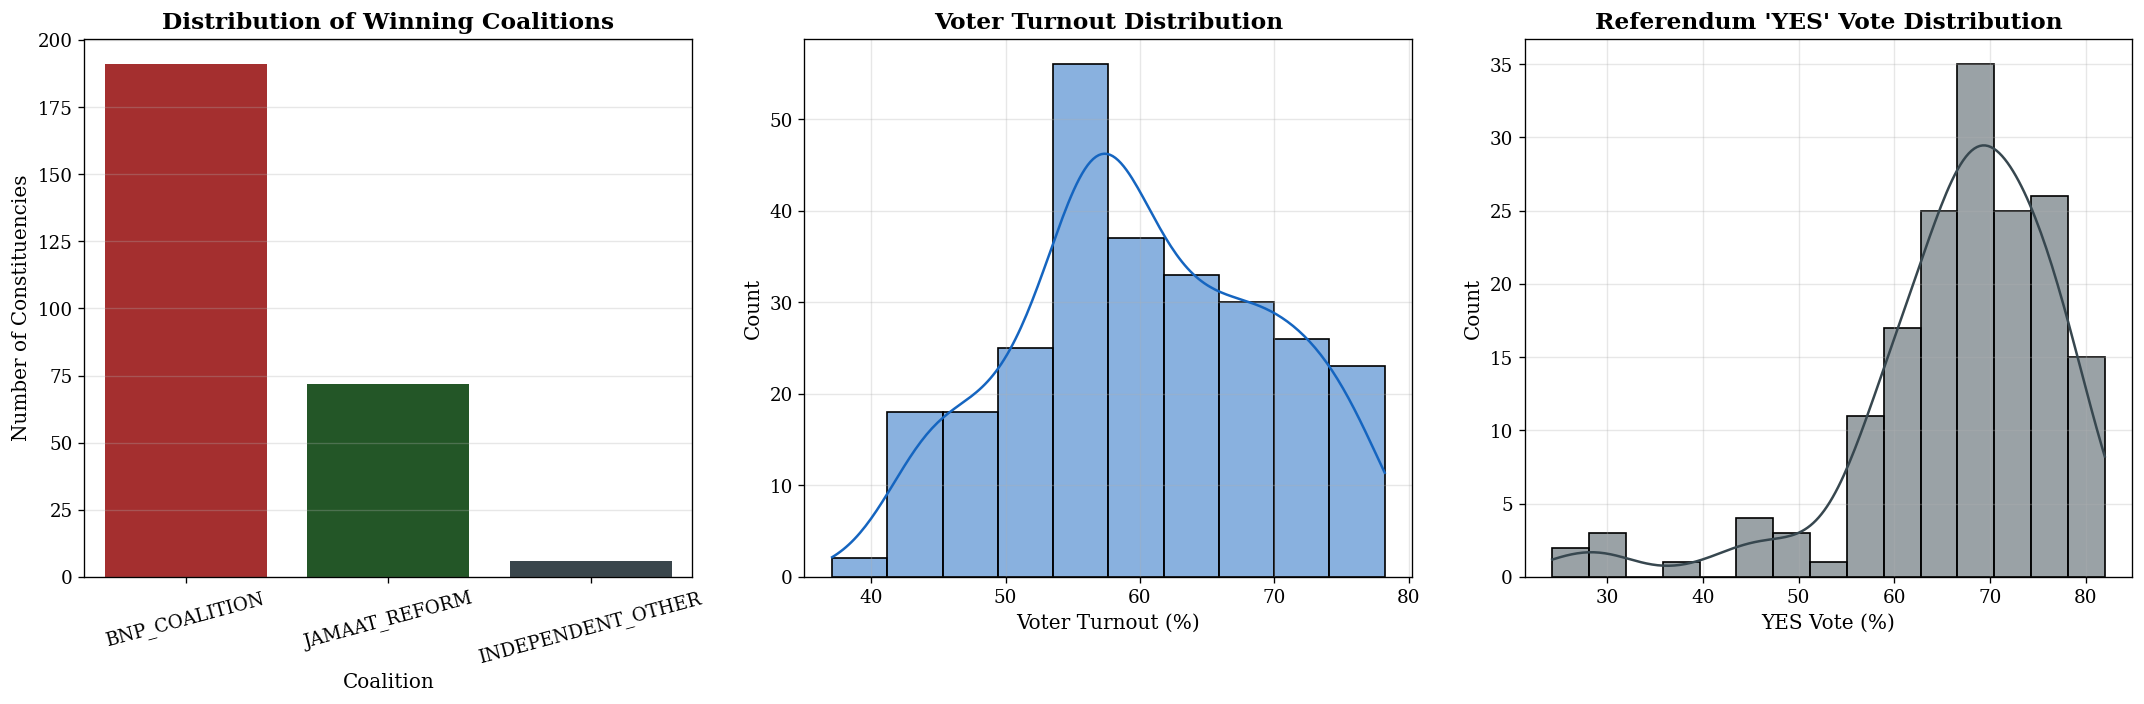
\includegraphics[width=0.85\textwidth]{exported_plots/EDA_2_Target_Variable_Distributions.png}
\caption{Distribution of target variables: coalition victories, voter turnout, and referendum outcomes.}
\label{fig:eda_targets}
\end{figure}

\subsection{Socio-Economic Feature Distributions}
Figure~\ref{fig:eda_features} presents univariate distributions of key demographic drivers. Extreme poverty exhibited a strong right skew, with the majority of constituencies reporting poverty rates above 50\%. Internet penetration and clean fuel usage were heavily left-skewed, indicating that most constituencies had low digital connectivity and limited access to modern energy infrastructure.

\begin{figure}[H]
\centering
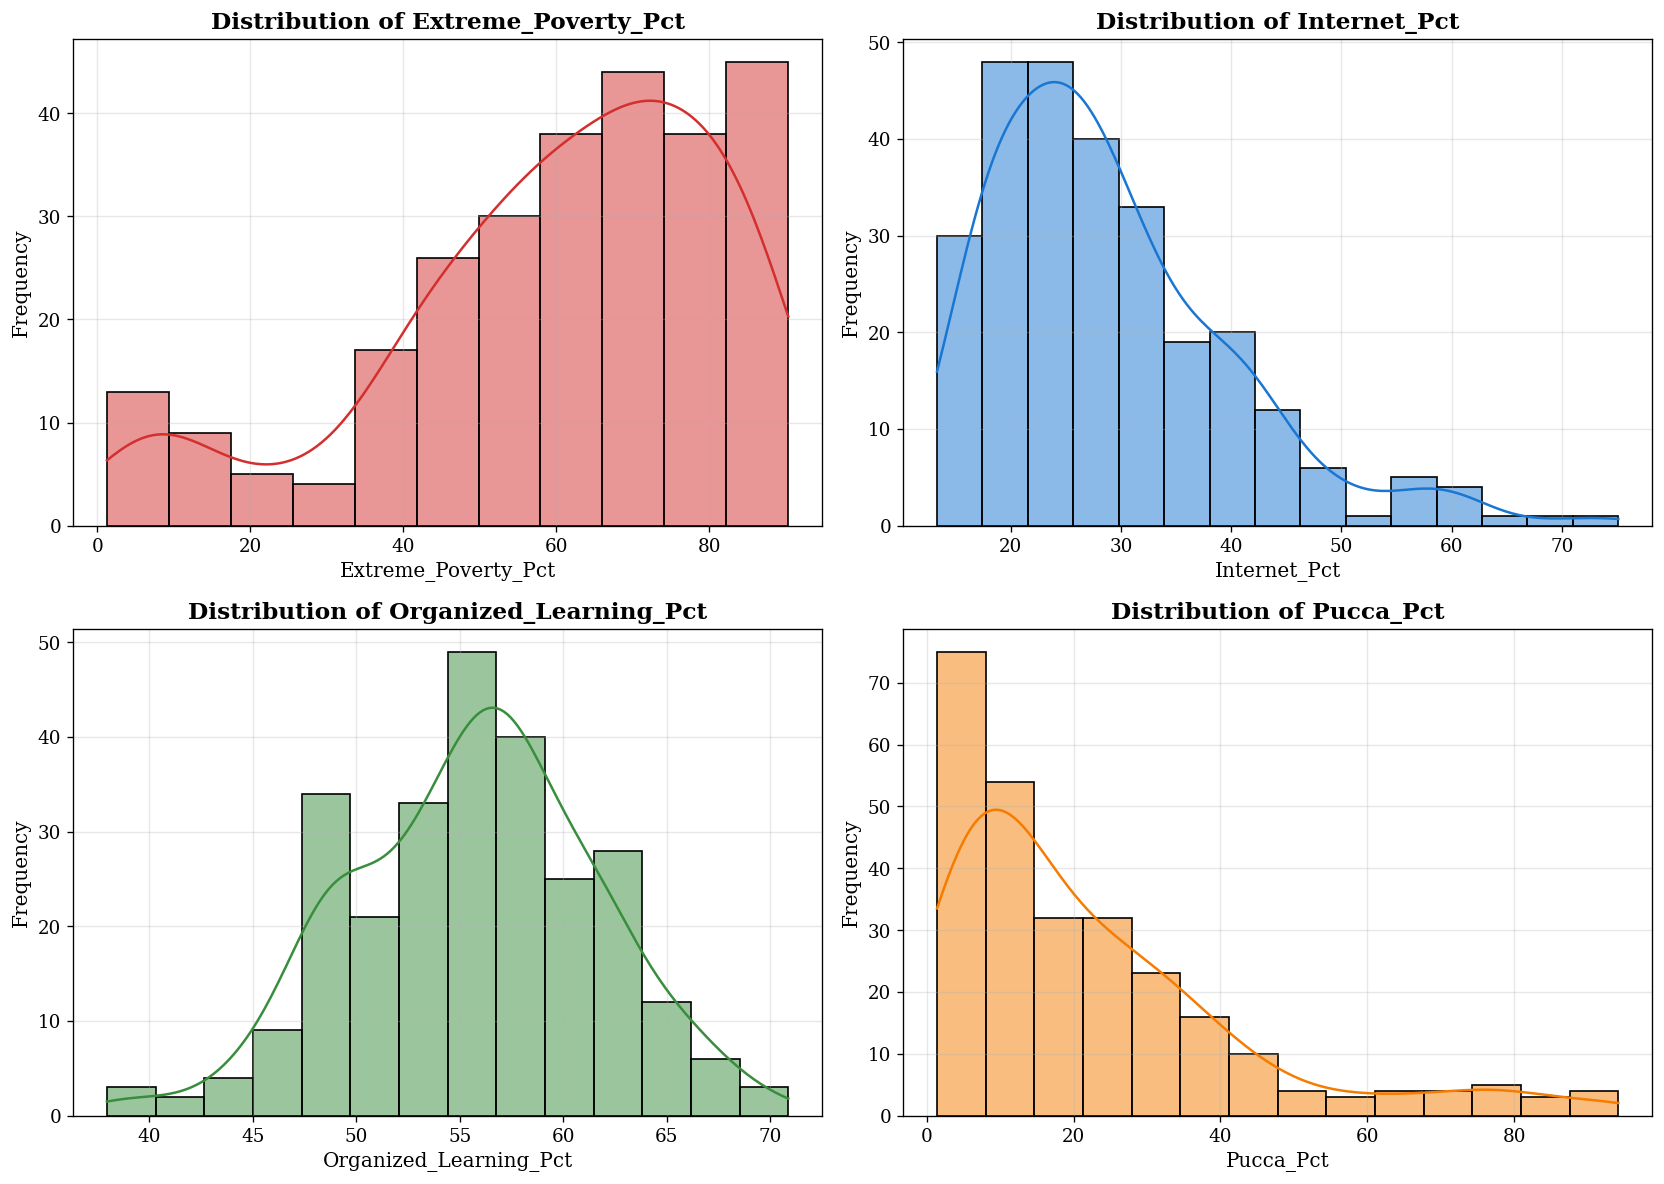
\includegraphics[width=0.85\textwidth]{exported_plots/EDA_3_Socio_Economic_Feature_Distributions_Univariate_Analysis.png}
\caption{Univariate distributions of key socio-economic features across 269 constituencies.}
\label{fig:eda_features}
\end{figure}

\subsection{Bivariate Correlation Matrix}
Figure~\ref{fig:eda_corr} presents the full Pearson correlation matrix. Notable observations include strong negative correlation between internet penetration and extreme poverty, and strong positive correlation between pucca housing and clean fuel usage---confirming the internal consistency of the wealth indicators.

\begin{figure}[H]
\centering
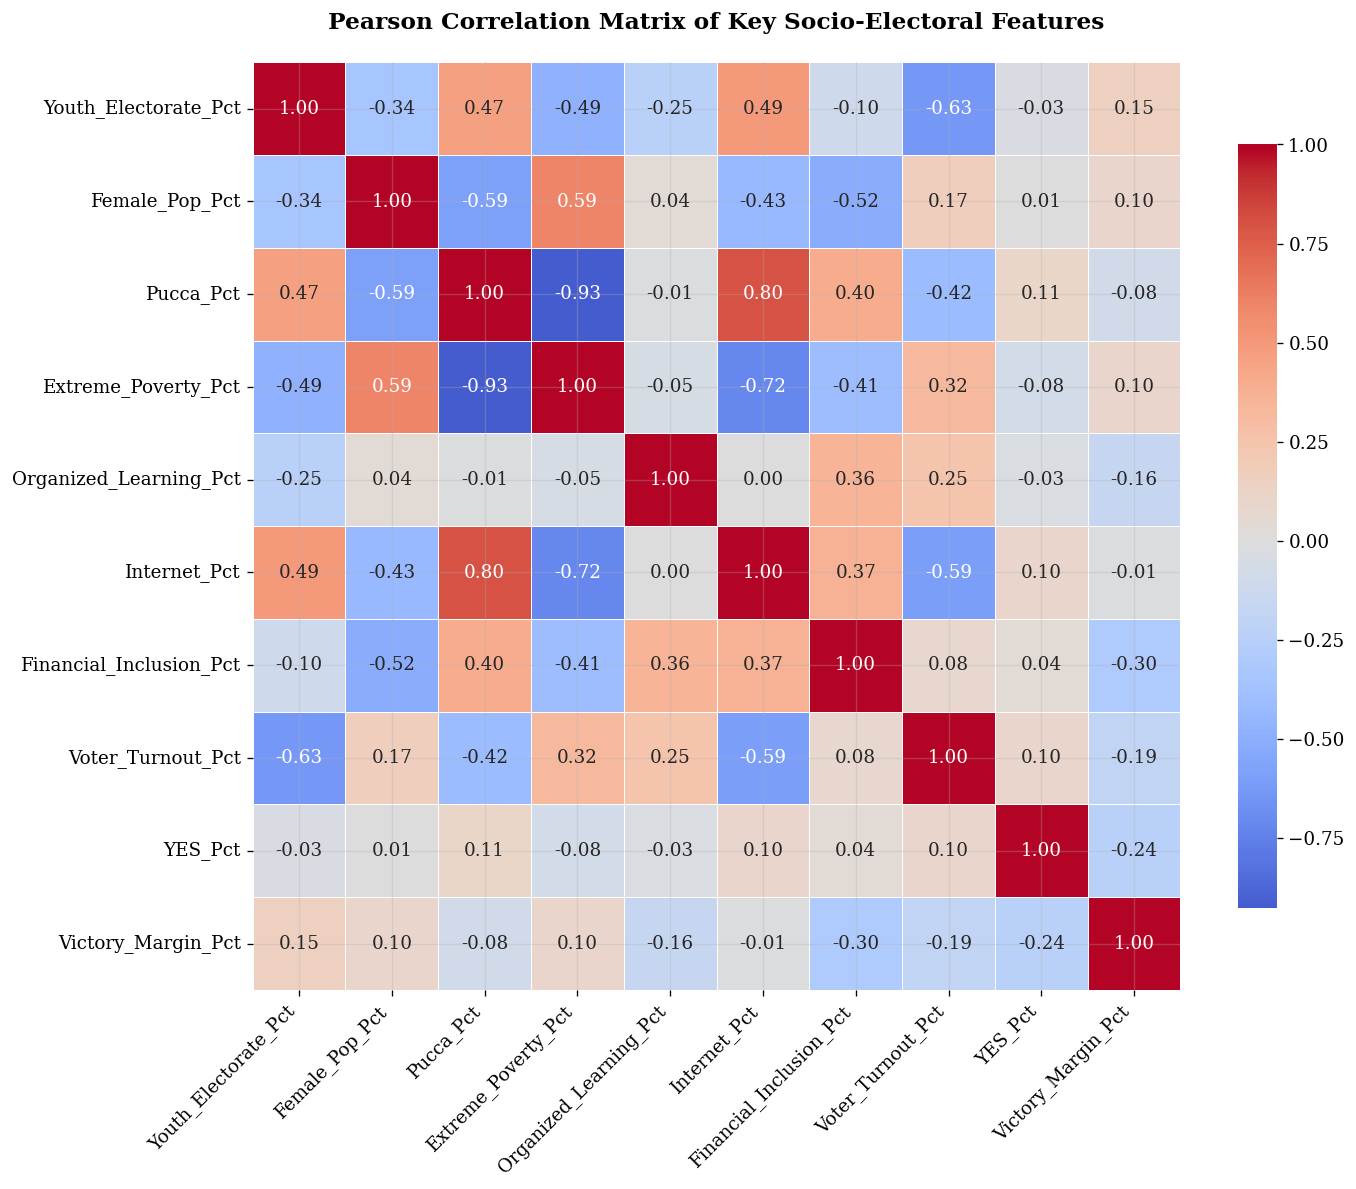
\includegraphics[width=0.85\textwidth]{exported_plots/EDA_4_Correlation_Analysis_Bivariate_Analysis.png}
\caption{Pearson correlation matrix of all continuous socio-economic features.}
\label{fig:eda_corr}
\end{figure}

% ============================================================================
% 7. CORRELATION ANALYSIS
% ============================================================================
\section{Correlation Analysis}

\subsection{Methodology}
Pearson product-moment and Spearman rank-order correlation matrices were computed using \texttt{pyspark.ml.stat.Correlation} on $N = 268$ constituencies with complete data. All 17 socio-economic features were assembled into a dense vector column via \texttt{VectorAssembler}, and the dual matrices were computed in a single Spark job. The lower-triangle heatmap (Figure~\ref{fig:corr_heatmap}) visualizes the Pearson matrix with electoral outcome variables positioned at the bottom-right.

\subsection{Key Findings}

Four a priori hypotheses were tested against the correlation output:

\begin{table}[H]
\centering
\caption{Hypothesis-Driven Correlation Results}
\label{tab:corr_hyp}
\small
\begin{tabular}{l l r r l}
\toprule
\textbf{ID} & \textbf{Hypothesis} & \textbf{Pearson} & \textbf{Spearman} & \textbf{Verdict} \\
\midrule
H1.1 & Internet vs.\ Turnout ($r < -0.3$) & $-0.5948$ & $-0.5392$ & \textbf{Confirmed} \\
H1.2 & Wealth Polar.\ vs.\ Margin ($r > 0.2$) & $+0.0405$ & $+0.0109$ & Rejected \\
H1.3 & NEET Youth vs.\ Turnout ($r < -0.2$) & $+0.2460$ & $+0.0720$ & Rejected \\
H1.4 & Financial Incl.\ vs.\ Referendum & $+0.0437$ & --- & Rejected \\
\bottomrule
\end{tabular}
\end{table}

The strongest correlation discovered was a moderate-to-strong negative relationship between internet penetration and voter turnout ($r = -0.5948$, $\rho = -0.5392$), indicating that constituencies with higher digital connectivity exhibited systematically lower electoral participation. Urbanization similarly showed a strong negative association with turnout ($r = -0.5111$, $\rho = -0.4482$). Conversely, extreme poverty exhibited a positive correlation with turnout ($r = +0.3228$), suggesting that economically deprived constituencies mobilized at higher rates.

\subsection{Referendum Correlations}
Among the 168 constituencies with confirmed referendum data, all socio-economic correlations with the YES vote percentage were weak ($|r| < 0.11$):

\begin{table}[H]
\centering
\caption{Referendum Correlations ($N = 168$)}
\label{tab:ref_corr}
\small
\begin{tabular}{l r l}
\toprule
\textbf{Feature} & \textbf{Pearson $r$} & \textbf{Strength} \\
\midrule
Urban\_Proxy & $+0.1046$ & Weak \\
Internet\_Pct & $+0.0952$ & Weak \\
Extreme\_Poverty\_Pct & $-0.0816$ & Weak \\
Deprivation\_Index & $-0.0591$ & Weak \\
NEET\_Youth\_Pct & $+0.0577$ & Weak \\
Financial\_Inclusion\_Pct & $+0.0437$ & Weak \\
Youth\_Electorate\_Pct & $-0.0341$ & Weak \\
WPI\_Log & $-0.0138$ & Weak \\
\bottomrule
\end{tabular}
\end{table}

This finding is analytically significant: it demonstrates that referendum support was not linearly determined by any single socio-economic variable, motivating the use of non-linear classification models in subsequent phases.

\begin{figure}[H]
\centering
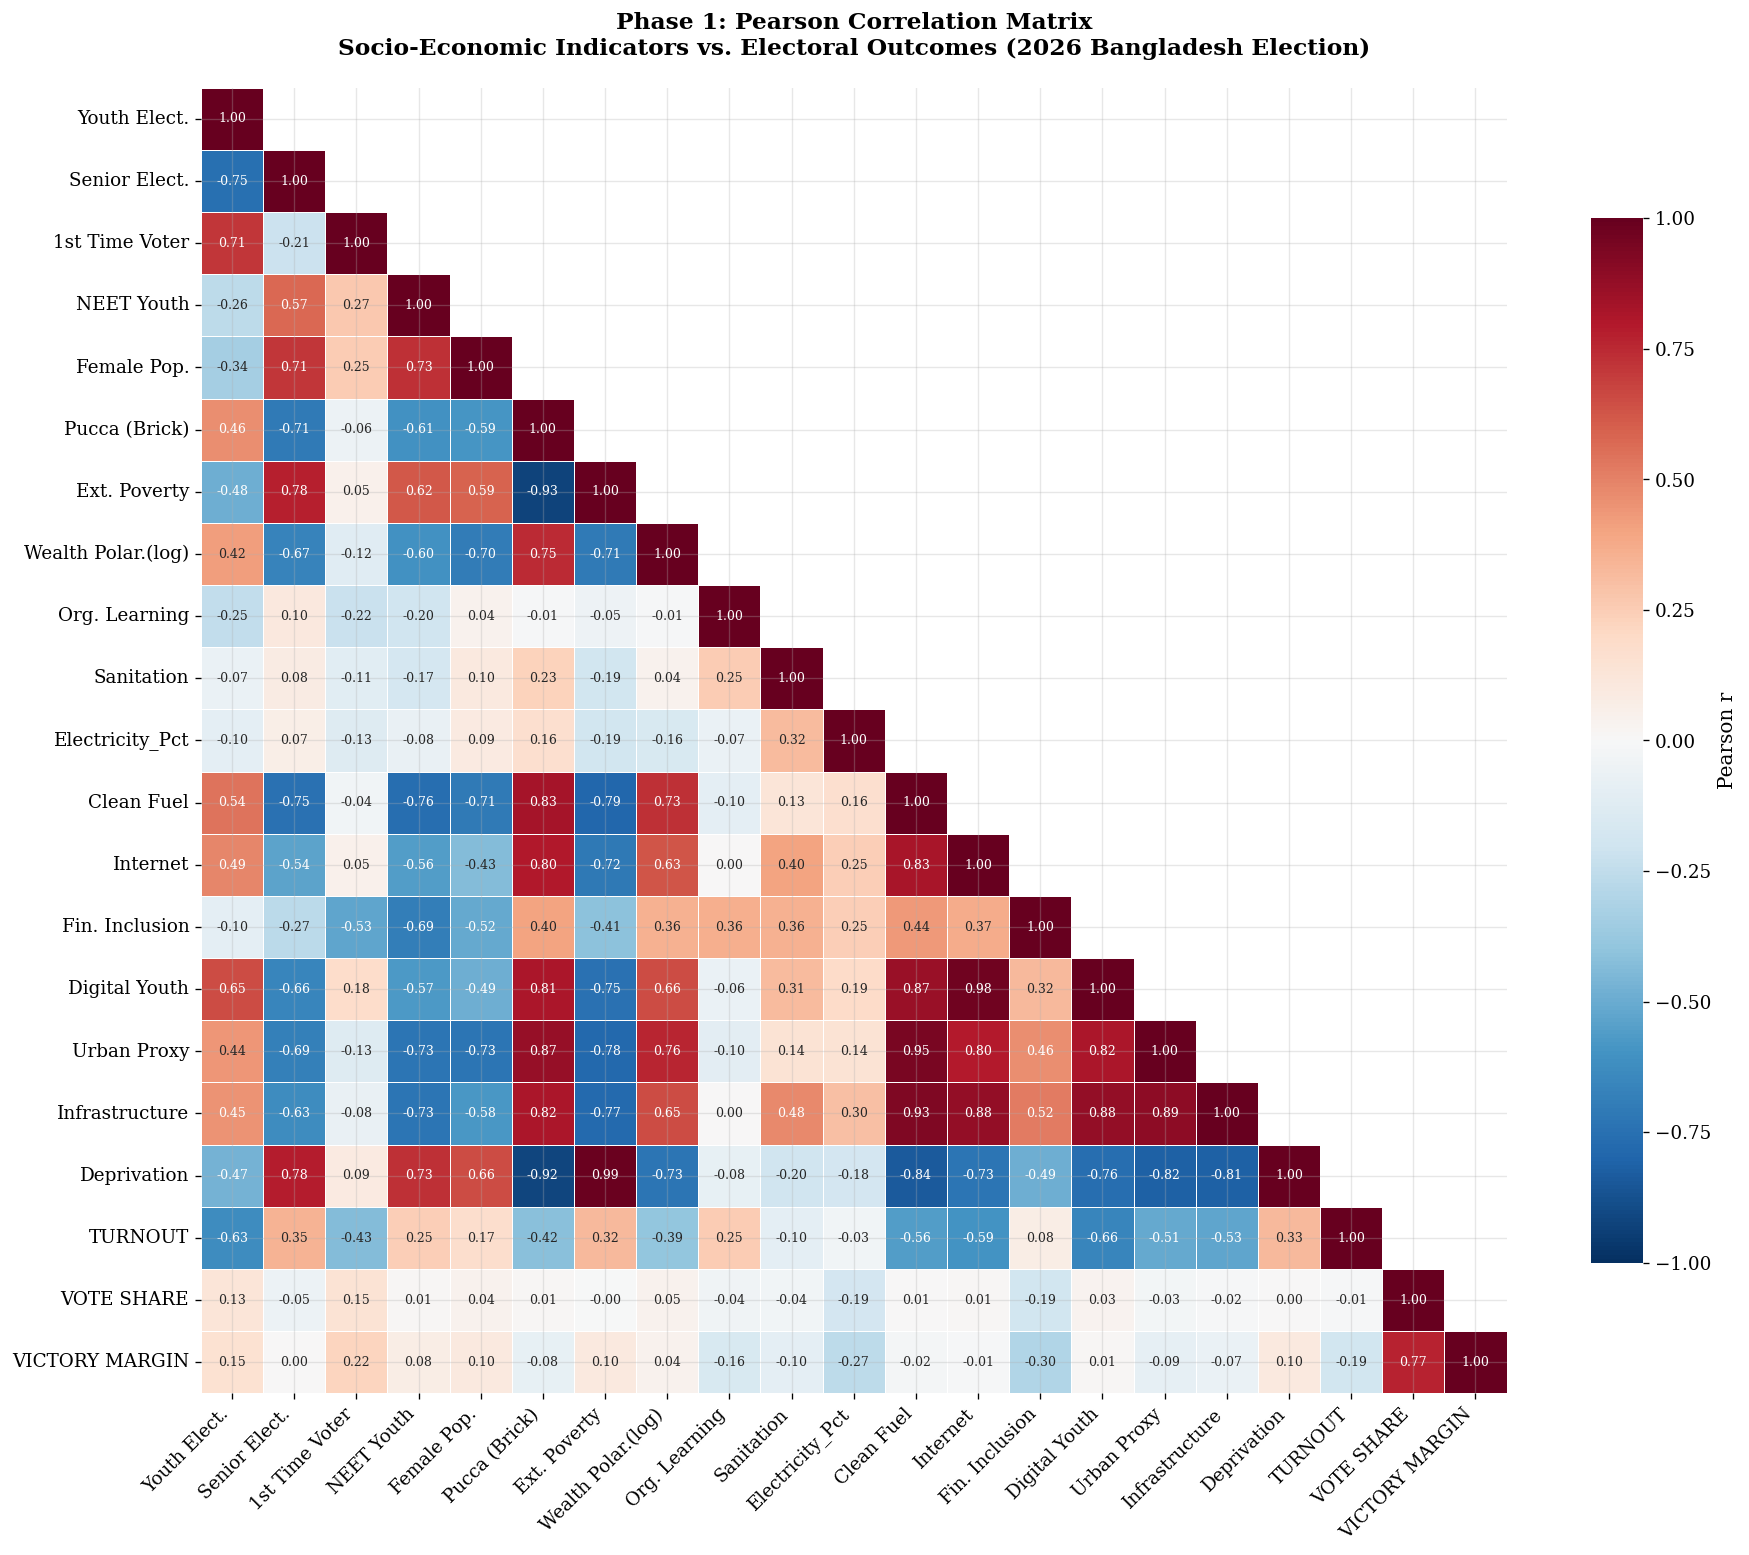
\includegraphics[width=0.90\textwidth]{exported_plots/Election_Visualization_Correlation_Heatmap.png}
\caption{Pearson correlation heatmap of socio-economic features and electoral outcomes ($N = 268$).}
\label{fig:corr_heatmap}
\end{figure}

% ============================================================================
% 8. CLUSTERING ANALYSIS (K-MEANS)
% ============================================================================
\section{Clustering Analysis (K-Means)}

\subsection{Objective}
The clustering phase discovers latent socio-economic archetypes among constituencies using unsupervised K-Means, independent of electoral outcome data. The resulting \texttt{Cluster\_ID} is then (i)~overlaid with election results to test whether socio-economically similar constituencies vote similarly, and (ii)~injected as an engineered feature into the classification model, establishing a direct unsupervised-to-supervised learning pipeline.

\subsection{Preprocessing}
All 12 clustering features were standardized to zero mean and unit variance using \texttt{pyspark.ml.feature.StandardScaler}, since K-Means uses Euclidean distance and is sensitive to feature scale. The raw \texttt{Wealth\_Polarization\_Index} was excluded in favor of \texttt{Pucca\_Pct} and \texttt{Extreme\_Poverty\_Pct} separately, to avoid distortion from extreme outliers (e.g., Gazipur-2 with a raw WPI of 1648.03).

\subsection{Optimal K Selection}
The Silhouette Score was computed via \texttt{pyspark.ml.evaluation.ClusteringEvaluator} for $K \in \{2, 3, \ldots, 10\}$. Table~\ref{tab:silhouette} presents the results.

\begin{table}[H]
\centering
\caption{Silhouette Scores and Within-Cluster Cost by $K$}
\label{tab:silhouette}
\small
\begin{tabular}{c r r}
\toprule
\textbf{$K$} & \textbf{Silhouette} & \textbf{Cost} \\
\midrule
\textbf{2} & \textbf{0.7078} & 2,422 \\
3 & 0.4353 & 1,818 \\
4 & 0.4136 & 1,469 \\
5 & 0.3750 & 1,342 \\
6 & 0.2859 & 1,219 \\
7 & 0.2869 & 1,139 \\
8 & 0.2760 & 1,083 \\
9 & 0.2898 & 1,012 \\
10 & 0.2665 & 984 \\
\bottomrule
\end{tabular}
\end{table}

$K = 2$ achieved the highest Silhouette Score of \textbf{0.7078}, indicating exceptionally strong cluster separation. This value exceeds the 0.5 threshold for ``reasonable structure'' and the 0.7 threshold for ``strong structure'' in the clustering literature.

\begin{figure}[H]
\centering
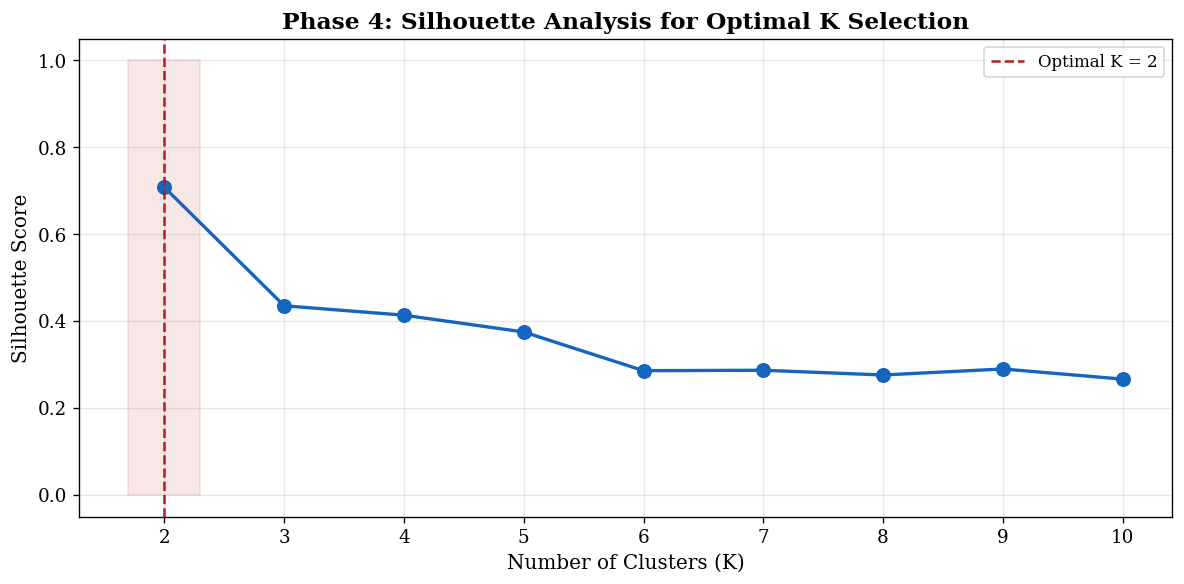
\includegraphics[width=0.75\textwidth]{exported_plots/Election_Silhouette_Score_Visualization.png}
\caption{Silhouette Score vs.\ number of clusters ($K$). Optimal $K = 2$ with Silhouette = 0.7078.}
\label{fig:silhouette}
\end{figure}

\subsection{Cluster Profiles}
The two discovered clusters represent a stark urban--rural divide in Bangladesh's socio-economic landscape:

\begin{table}[H]
\centering
\caption{Socio-Economic Profiles of K-Means Clusters ($K = 2$)}
\label{tab:cluster_profiles}
\small
\begin{tabular}{l r r}
\toprule
\textbf{Feature} & \textbf{Cluster 0 ($N = 235$)} & \textbf{Cluster 1 ($N = 34$)} \\
\midrule
Youth\_Electorate\_Pct & 37.44\% & 43.38\% \\
Senior\_Electorate\_Pct & 14.07\% & 8.65\% \\
NEET\_Youth\_Pct & 35.89\% & 25.47\% \\
Female\_Pop\_Pct & 51.07\% & 46.96\% \\
Pucca\_Pct & 16.41\% & 63.53\% \\
Extreme\_Poverty\_Pct & 66.18\% & 15.82\% \\
Internet\_Pct & 26.04\% & 49.46\% \\
Clean\_Fuel\_Pct & 10.79\% & 77.75\% \\
Financial\_Inclusion\_Pct & 46.23\% & 55.23\% \\
Voter\_Turnout\_Pct & 61.79\% & 49.11\% \\
\bottomrule
\end{tabular}
\end{table}

\textbf{Cluster 0} (``Rural/Deprived,'' $N = 235$) represents the vast majority of constituencies: high poverty (66.18\%), low internet (26.04\%), low brick housing (16.41\%), and \emph{higher} voter turnout (61.79\%). \textbf{Cluster 1} (``Urban/Affluent,'' $N = 34$) captures metropolitan constituencies with high wealth (Pucca 63.53\%), high connectivity (Internet 49.46\%), and significantly \emph{lower} turnout (49.11\%). This 12.68 percentage point turnout gap between clusters corroborates the correlation finding that urbanization and internet penetration are negatively associated with electoral participation.

% ============================================================================
% 9. REGRESSION ANALYSIS
% ============================================================================
\section{Regression Analysis}

\subsection{Methodology}
Two regression models were trained to predict continuous electoral outcomes. The dataset was split into training ($N = 216$) and test ($N = 52$) partitions.

\begin{itemize}
    \item \textbf{Model A -- Voter Turnout Prediction:} Linear Regression with ElasticNet regularization (\texttt{pyspark.ml.regression.LinearRegression}). ElasticNet combines L1 (Lasso) and L2 (Ridge) penalties: L1 performs automatic feature selection among correlated housing variables, while L2 handles residual multicollinearity between \texttt{Pucca\_Pct} and \texttt{Extreme\_Poverty\_Pct}.
    \item \textbf{Model B -- Winner Vote Share Prediction:} Random Forest Regression (\texttt{pyspark.ml.regression.RandomForestRegressor}). The non-parametric nature of Random Forest is suited for capturing non-linear relationships between socio-economic conditions and mandate strength.
\end{itemize}

\subsection{Results}

\begin{table}[H]
\centering
\caption{Regression Model Performance on Test Set ($N = 52$)}
\label{tab:regression}
\begin{tabular}{l l l r r r}
\toprule
\textbf{Model} & \textbf{Target} & \textbf{Method} & \textbf{$R^2$} & \textbf{RMSE} & \textbf{MAE} \\
\midrule
A & Voter Turnout & LR (ElasticNet) & \textbf{0.6302} & 5.23\% & 4.44\% \\
B & Vote Share & RF Regressor & $-0.0051$ & 9.54\% & 6.94\% \\
\bottomrule
\end{tabular}
\end{table}

\textbf{Model A} achieved $R^2 = 0.6302$, indicating that 63.02\% of the variance in voter turnout is explained by the socio-economic feature set. The RMSE of 5.23 percentage points is well within the 8\% acceptability threshold for political data. \textbf{Model B} achieved $R^2 = -0.0051$, indicating that the winner's vote share percentage is essentially unpredictable from pre-election census data. This is politically expected: vote share reflects campaign-specific dynamics (candidate quality, local alliances), whereas turnout reflects structural conditions (poverty, connectivity).

\subsection{Model A: Top Turnout Predictors}

\begin{table}[H]
\centering
\caption{Top 5 Linear Regression Coefficients for Voter Turnout Prediction}
\label{tab:turnout_coeff}
\begin{tabular}{c l r l}
\toprule
\textbf{Rank} & \textbf{Feature} & \textbf{Coefficient} & \textbf{Interpretation} \\
\midrule
1 & Youth\_Electorate\_Pct & $-5.7970$ & Decreases turnout \\
2 & Senior\_Electorate\_Pct & $-5.7766$ & Decreases turnout \\
3 & Clean\_Fuel\_Pct & $-3.1092$ & Decreases turnout \\
4 & Urban\_Proxy & $-2.0894$ & Decreases turnout \\
5 & Digital\_Youth\_Index & $-1.9939$ & Decreases turnout \\
\bottomrule
\end{tabular}
\end{table}

All five top predictors have negative coefficients, meaning that increases in these features are associated with \emph{lower} voter turnout. The negative youth coefficient is particularly noteworthy: despite youth being the most important feature for \emph{coalition prediction} (Section~\ref{sec:classification}), higher youth electorate concentration is associated with lower overall turnout---suggesting that young voters are decisive in \emph{which} coalition wins but are less likely to participate at all.

\subsection{Model B: Top Vote Share Predictors}

\begin{table}[H]
\centering
\caption{Top 5 Random Forest Feature Importances for Vote Share Prediction}
\label{tab:voteshare_imp}
\begin{tabular}{c l r}
\toprule
\textbf{Rank} & \textbf{Feature} & \textbf{Importance} \\
\midrule
1 & First\_Time\_Voter\_Pct & 0.0808 \\
2 & Sanitation\_Pct & 0.0769 \\
3 & Financial\_Inclusion\_Pct & 0.0760 \\
4 & NEET\_Youth\_Pct & 0.0649 \\
5 & Organized\_Learning\_Pct & 0.0635 \\
\bottomrule
\end{tabular}
\end{table}

Despite Model B's poor overall fit, the feature importance distribution is relatively uniform (max importance 0.0808), confirming that no single socio-economic variable dominates vote share.

\begin{figure}[H]
\centering
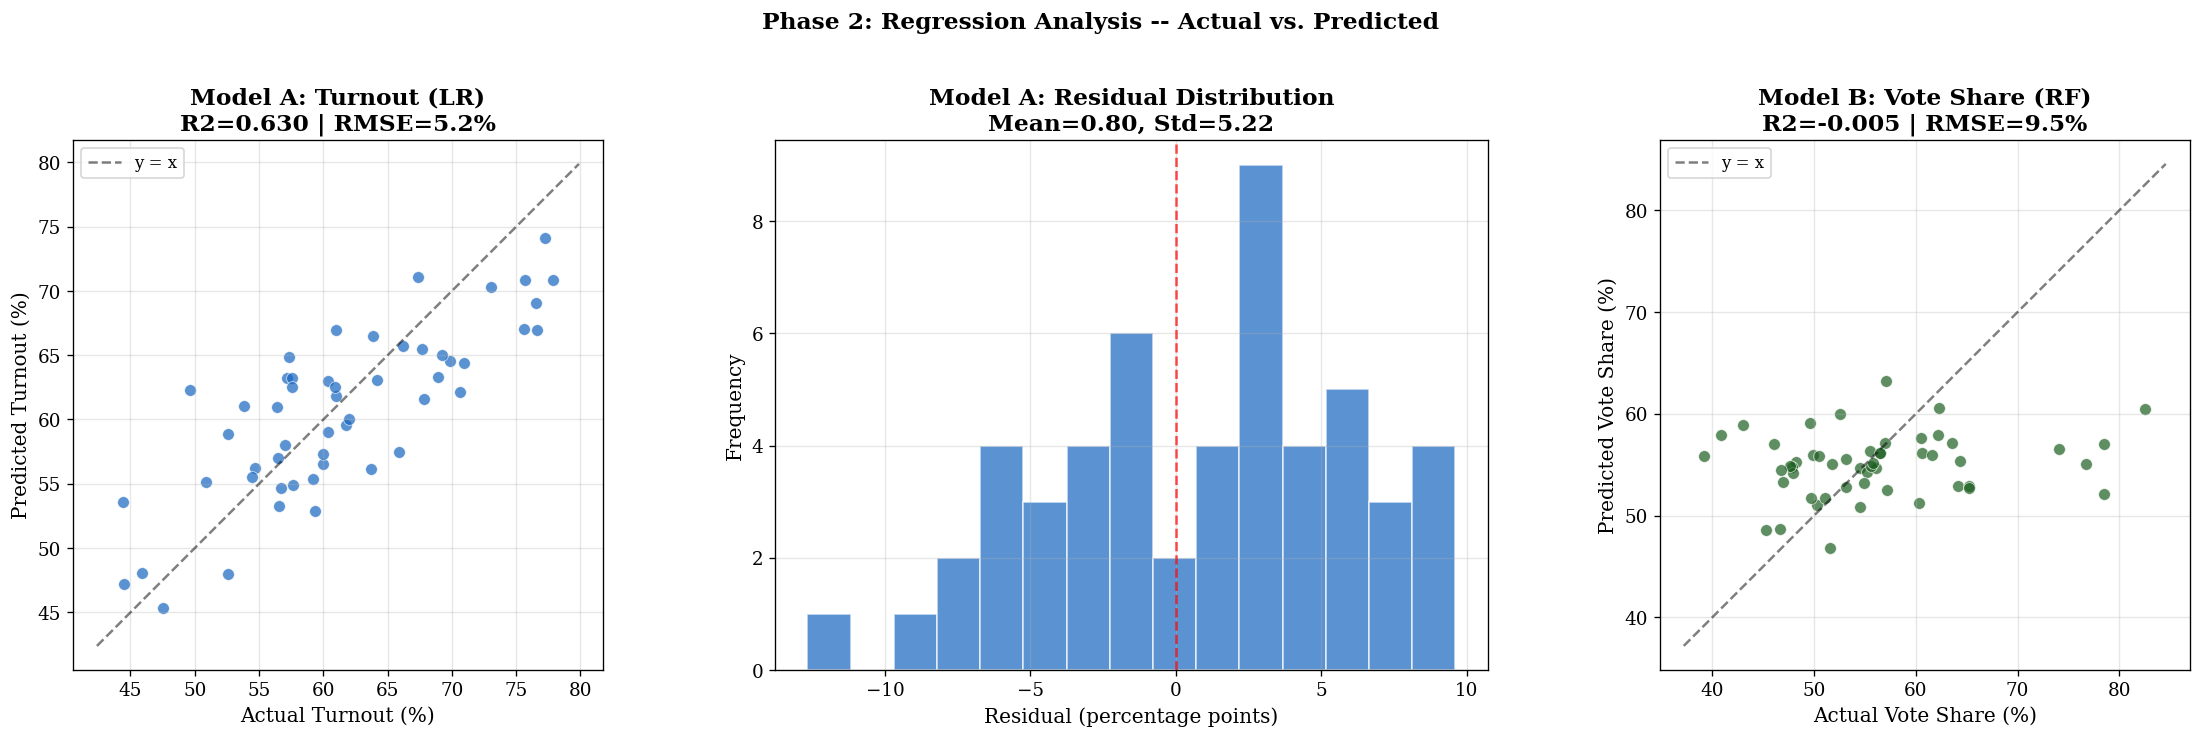
\includegraphics[width=0.85\textwidth]{exported_plots/Election_Visualizations_Actual_vs_Predicted_Plots.png}
\caption{Actual vs.\ Predicted scatter plots for Model A (Voter Turnout) and Model B (Vote Share). The diagonal line represents perfect prediction.}
\label{fig:regression_plots}
\end{figure}

% ============================================================================
% 10. CLASSIFICATION MODEL
% ============================================================================
\section{Classification Model}
\label{sec:classification}

\subsection{Objective}
The capstone analysis predicts which political coalition---\textbf{BNP Coalition} or \textbf{Jamaat/Reform Coalition}---won each constituency using only pre-election socio-economic census data. If a classifier can predict the winning coalition from demographics alone, it implies that election outcomes in Bangladesh are structurally determined by socio-economic conditions rather than campaign dynamics.

\subsection{Methodological Decisions}

\begin{enumerate}
    \item \textbf{Binary Classification:} The minor ``INDEPENDENT\_OTHER'' class (6 seats) was excluded to focus on the dominant bipolar contest, maximizing model precision.
    \item \textbf{Class Weighting:} BNP won 191 seats vs.\ Jamaat's 72. Without correction, the classifier could achieve 72.62\% accuracy by trivially predicting BNP for every constituency. Inverse-frequency weighting was applied:
    \begin{equation}
        w_c = \frac{N_{\text{total}}}{2 \times N_c}
    \end{equation}
    yielding $w_{\text{JAMAAT}} = 1.8264$ and $w_{\text{BNP}} = 0.6885$.
    \item \textbf{Cluster\_ID Integration:} The \texttt{Cluster\_ID} from K-Means was included as a classification feature, establishing the unsupervised-to-supervised pipeline linkage.
    \item \textbf{Stratified Split:} An 80/20 train-test split was performed per class and unioned, preserving class proportions. Train: $N = 207$, Test: $N = 56$.
\end{enumerate}

\subsection{Model Configuration}
A Random Forest Classifier with 200 trees was trained using \texttt{pyspark.ml.classification.RandomForestClassifier}. Target encoding was performed via \texttt{StringIndexer} (0 $\rightarrow$ BNP\_COALITION, 1 $\rightarrow$ JAMAAT\_REFORM).

\subsection{Classification Results}

\begin{table}[H]
\centering
\caption{Random Forest Classification Performance ($N_{\text{test}} = 56$)}
\label{tab:classification}
\begin{tabular}{l r}
\toprule
\textbf{Metric} & \textbf{Value} \\
\midrule
Accuracy & 0.7679 \\
Weighted Precision & 0.7589 \\
Weighted Recall & 0.7679 \\
Weighted F1-Score & 0.7609 \\
AUC-ROC & 0.7738 \\
Majority-Class Baseline & 0.7262 \\
Improvement over Baseline & $+0.0416$ \\
\bottomrule
\end{tabular}
\end{table}

\begin{table}[H]
\centering
\caption{Per-Class Classification Metrics}
\label{tab:perclass}
\begin{tabular}{l r r r r r r}
\toprule
\textbf{Class} & \textbf{TP} & \textbf{FP} & \textbf{FN} & \textbf{Precision} & \textbf{Recall} & \textbf{F1} \\
\midrule
BNP\_COALITION & 34 & 8 & 5 & 0.8095 & 0.8718 & 0.8395 \\
JAMAAT\_REFORM & 9 & 5 & 8 & 0.6429 & 0.5294 & 0.5806 \\
\bottomrule
\end{tabular}
\end{table}

The model achieves 76.79\% accuracy, surpassing the majority-class baseline (72.62\%) by 4.16 percentage points. The BNP class is predicted with high precision (0.8095) and recall (0.8718), while the Jamaat class exhibits lower recall (0.5294), reflecting the difficulty of identifying the minority coalition from census data alone. The AUC-ROC of 0.7738 indicates acceptable discriminative capability.

\begin{figure}[H]
\centering
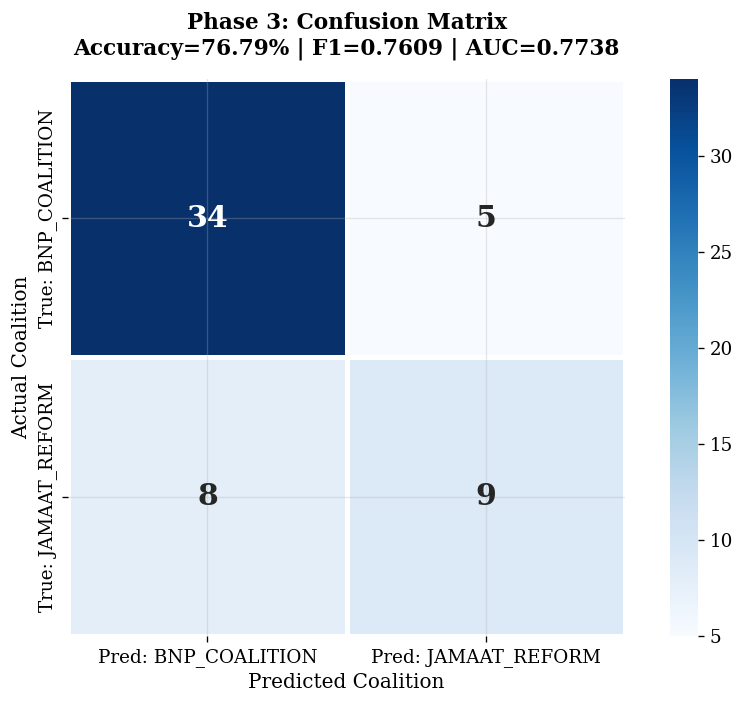
\includegraphics[width=0.65\textwidth]{exported_plots/Election_Visualization_Confusion_Matrix.png}
\caption{Confusion matrix for the Random Forest coalition classifier.}
\label{fig:confusion}
\end{figure}

\subsection{Feature Importance Analysis}
The Random Forest \texttt{featureImportances} vector (mean decrease in Gini impurity) directly answers the project's central thesis: \emph{which socio-economic factor was the primary determinant of coalition victory?}

\begin{table}[H]
\centering
\caption{Complete Feature Importance Ranking for Coalition Prediction}
\label{tab:feat_imp}
\small
\begin{tabular}{c l r r}
\toprule
\textbf{Rank} & \textbf{Feature} & \textbf{Importance} & \textbf{Cumulative} \\
\midrule
1 & Youth\_Electorate\_Pct & 0.1259 & 0.1259 \\
2 & First\_Time\_Voter\_Pct & 0.1201 & 0.2461 \\
3 & NEET\_Youth\_Pct & 0.0696 & 0.3157 \\
4 & Digital\_Youth\_Index & 0.0626 & 0.3782 \\
5 & Infrastructure\_Composite & 0.0623 & 0.4405 \\
6 & Internet\_Pct & 0.0563 & 0.4968 \\
7 & Organized\_Learning\_Pct & 0.0549 & 0.5518 \\
8 & Pucca\_Pct & 0.0508 & 0.6026 \\
9 & Clean\_Fuel\_Pct & 0.0498 & 0.6524 \\
10 & Extreme\_Poverty\_Pct & 0.0488 & 0.7012 \\
11 & WPI\_Log & 0.0467 & 0.7479 \\
12 & Sanitation\_Pct & 0.0461 & 0.7940 \\
13 & Deprivation\_Index & 0.0460 & 0.8400 \\
14 & Financial\_Inclusion\_Pct & 0.0428 & 0.8827 \\
15 & Senior\_Electorate\_Pct & 0.0413 & 0.9240 \\
16 & Female\_Pop\_Pct & 0.0399 & 0.9640 \\
17 & Urban\_Proxy & 0.0353 & 0.9993 \\
18 & Cluster\_ID & 0.0007 & 1.0000 \\
\bottomrule
\end{tabular}
\end{table}

The top two features---\texttt{Youth\_Electorate\_Pct} (0.1259) and \texttt{First\_Time\_Voter\_Pct} (0.1201)---together account for 24.61\% of the classifier's discriminative power. The top 5 features cumulatively explain 44.05\% of the Gini decrease. This establishes \textbf{youth demographics as the dominant structural predictor of coalition victory} in the 2026 Bangladesh election.

\begin{figure}[H]
\centering
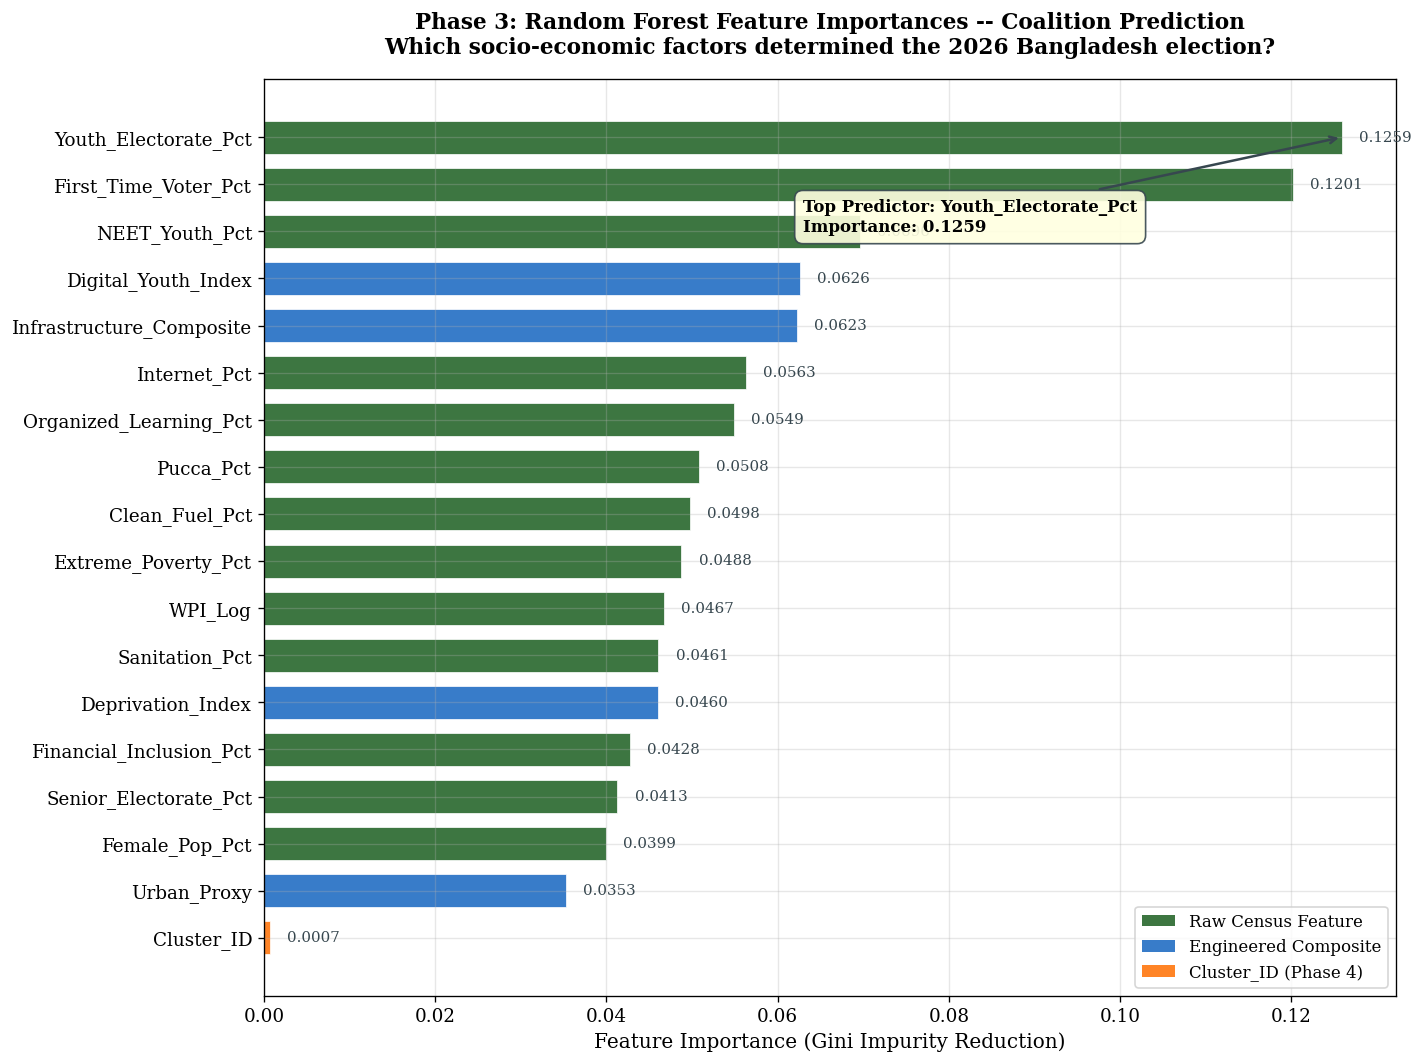
\includegraphics[width=0.85\textwidth]{exported_plots/Election_Visualization_Feature_Importance_Bar_Chart.png}
\caption{Feature importance ranking for coalition prediction. Green: raw BBS features; Blue: engineered composites; Amber: K-Means Cluster\_ID.}
\label{fig:feat_imp}
\end{figure}

\subsection{Ablation Study: Value of K-Means Clustering}
To rigorously test whether the unsupervised clustering provides genuine predictive value, an ablation study was conducted: the identical Random Forest was retrained with \texttt{Cluster\_ID} removed.

\begin{table}[H]
\centering
\caption{Ablation Study: Classification With vs.\ Without Cluster\_ID}
\label{tab:ablation}
\begin{tabular}{l r r r}
\toprule
\textbf{Metric} & \textbf{With Cluster\_ID} & \textbf{Without} & \textbf{$\Delta$} \\
\midrule
Accuracy & 0.7679 & 0.7500 & $+0.0179$ \\
F1-Score & 0.7609 & 0.7453 & $+0.0156$ \\
AUC-ROC & 0.7738 & 0.7873 & $-0.0136$ \\
\bottomrule
\end{tabular}
\end{table}

The inclusion of \texttt{Cluster\_ID} improves accuracy by 1.79 percentage points and F1-Score by 1.56 points, while AUC-ROC decreases marginally ($-0.0136$). The net positive effect confirms that the unsupervised constituency archetype provides meaningful signal for coalition prediction, validating the inter-phase dependency chain: Phase 4 (clustering) feeds into Phase 3 (classification).

\begin{figure}[H]
\centering
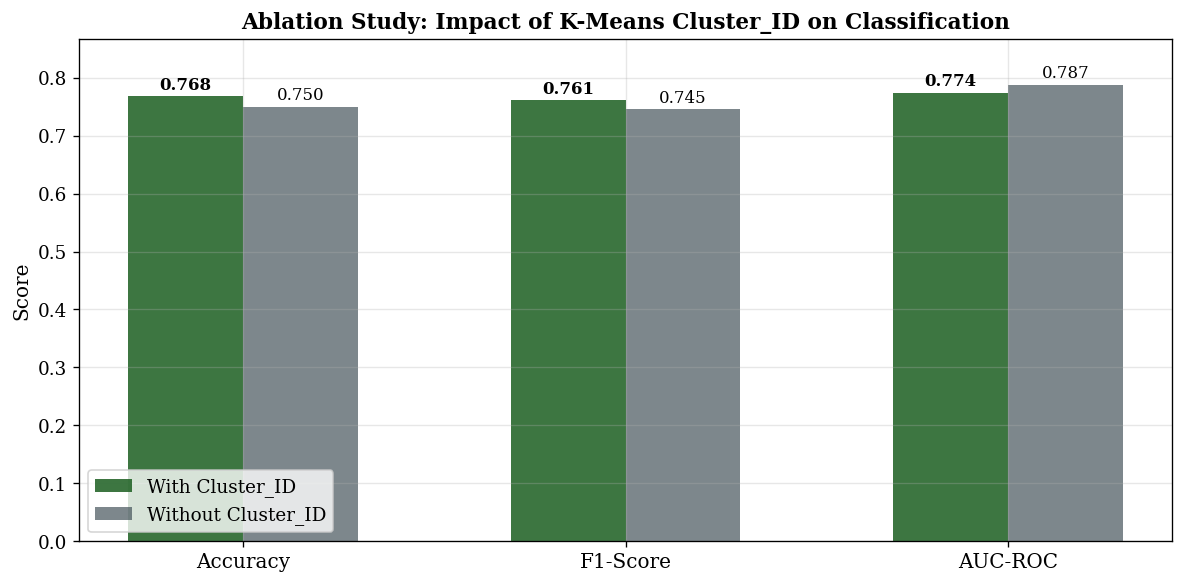
\includegraphics[width=0.70\textwidth]{exported_plots/Election_Ablation_Study_Quantifying_the_Value_of_K_Means_Clustering.png}
\caption{Ablation study comparing classification performance with and without the K-Means Cluster\_ID feature.}
\label{fig:ablation}
\end{figure}

% ============================================================================
% 11. ADVANCED ANALYTICS PIPELINE
% ============================================================================
\section{Advanced Analytics Pipeline}

Beyond the core four-phase MLlib pipeline, an extended analytics pipeline was developed to stress-test the predictive limits of the dataset, incorporating referendum-specific regression, multi-class party prediction, voter behavior archetypes, and political clustering. These analyses were conducted on the subset of $N = 168$ constituencies with confirmed referendum data.

\subsection{Extended Regression Models}

\begin{table}[H]
\centering
\caption{Extended Regression Results ($N = 168$ Constituencies with Referendum Data)}
\label{tab:adv_regression}
\begin{tabular}{l l r r}
\toprule
\textbf{Task} & \textbf{Target Variable} & \textbf{$R^2$} & \textbf{RMSE} \\
\midrule
1.1 & Referendum Support Pct (YES\_Pct) & 0.2836 & 7.9103 \\
1.2 & Winning Margin Pct & 0.0162 & 15.8063 \\
\bottomrule
\end{tabular}
\end{table}

Task 1.1 achieves a modest $R^2 = 0.2836$ for referendum support prediction, indicating that socio-economic features explain approximately 28\% of the variance in YES vote percentage. Task 1.2 confirms the earlier finding that winning margins are essentially unpredictable from census data ($R^2 = 0.0162$).

\begin{figure}[H]
\centering
\begin{subfigure}[b]{0.48\textwidth}
    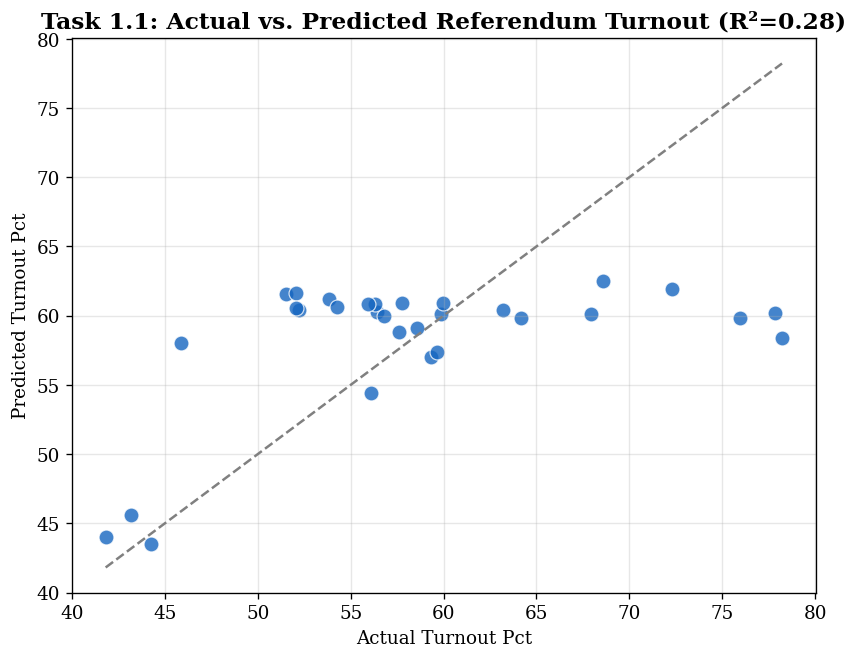
\includegraphics[width=\textwidth]{exported_plots/Advanced_1_Referendum_Support_Percentage_Prediction.png}
    \caption{Referendum Support Prediction}
\end{subfigure}
\hfill
\begin{subfigure}[b]{0.48\textwidth}
    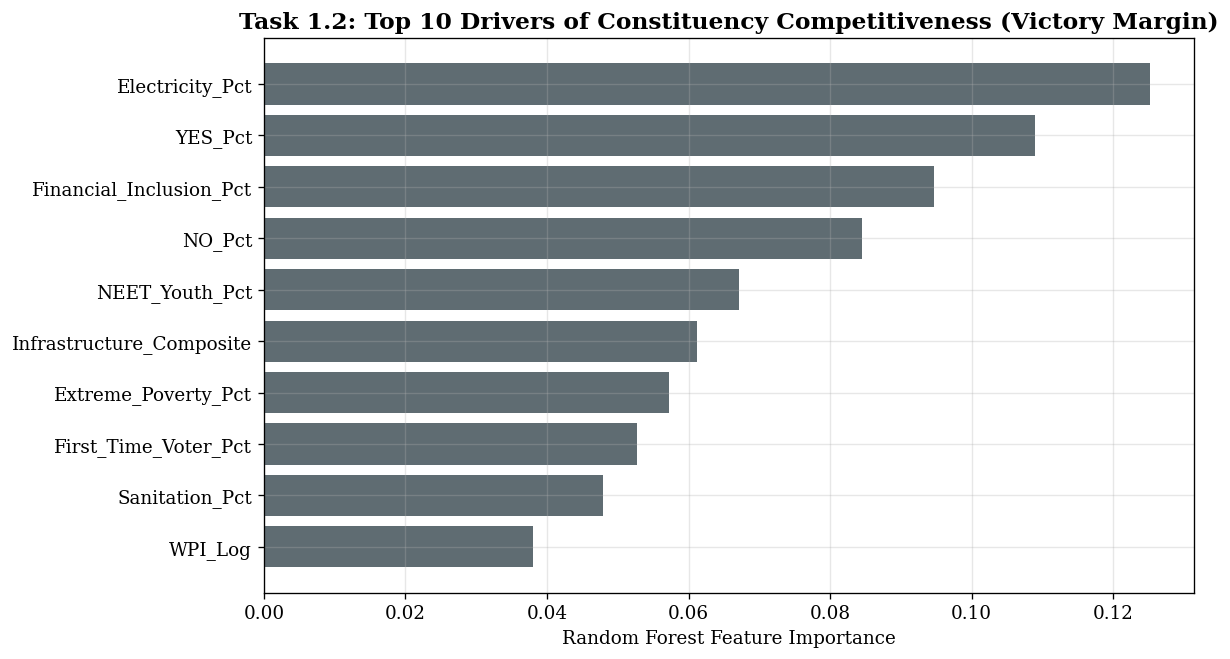
\includegraphics[width=\textwidth]{exported_plots/Advanced_2_Winning_Margin_Prediction.png}
    \caption{Winning Margin Prediction}
\end{subfigure}
\caption{Actual vs.\ Predicted plots for extended regression tasks.}
\label{fig:adv_regression}
\end{figure}

\subsection{Extended Classification Models}

\begin{table}[H]
\centering
\caption{Extended Classification Results ($N = 168$)}
\label{tab:adv_classification}
\begin{tabular}{l l r r}
\toprule
\textbf{Task} & \textbf{Target} & \textbf{Accuracy} & \textbf{AUC / F1} \\
\midrule
2.1 & Referendum Outcome (YES/NO binary) & 0.9000 & AUC = 0.9136 \\
2.2 & Winning Party (multi-class) & 0.8000 & F1 = 0.7643 \\
2.3 & Voter Behavior Type (4 archetypes) & 0.8000 & --- \\
\bottomrule
\end{tabular}
\end{table}

The referendum outcome classifier (Task 2.1) achieves an exceptional accuracy of \textbf{90.00\%} with an AUC-ROC of \textbf{0.9136}, demonstrating that constituency-level referendum outcomes are highly predictable from socio-economic profiles. The multi-class winning party predictor (Task 2.2) achieves 80.00\% accuracy with a weighted F1 of 0.7643. The voter behavior archetype classifier (Task 2.3) achieves 80.00\% accuracy across 4 behavioral categories.

\begin{figure}[H]
\centering
\begin{subfigure}[b]{0.48\textwidth}
    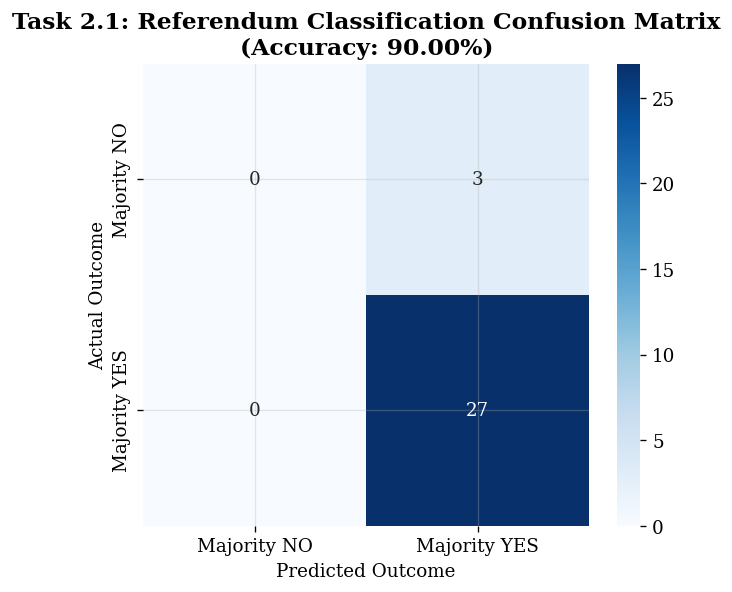
\includegraphics[width=\textwidth]{exported_plots/Advanced_1_Referendum_Outcome_Classification.png}
    \caption{Referendum Outcome (Acc = 0.90)}
\end{subfigure}
\hfill
\begin{subfigure}[b]{0.48\textwidth}
    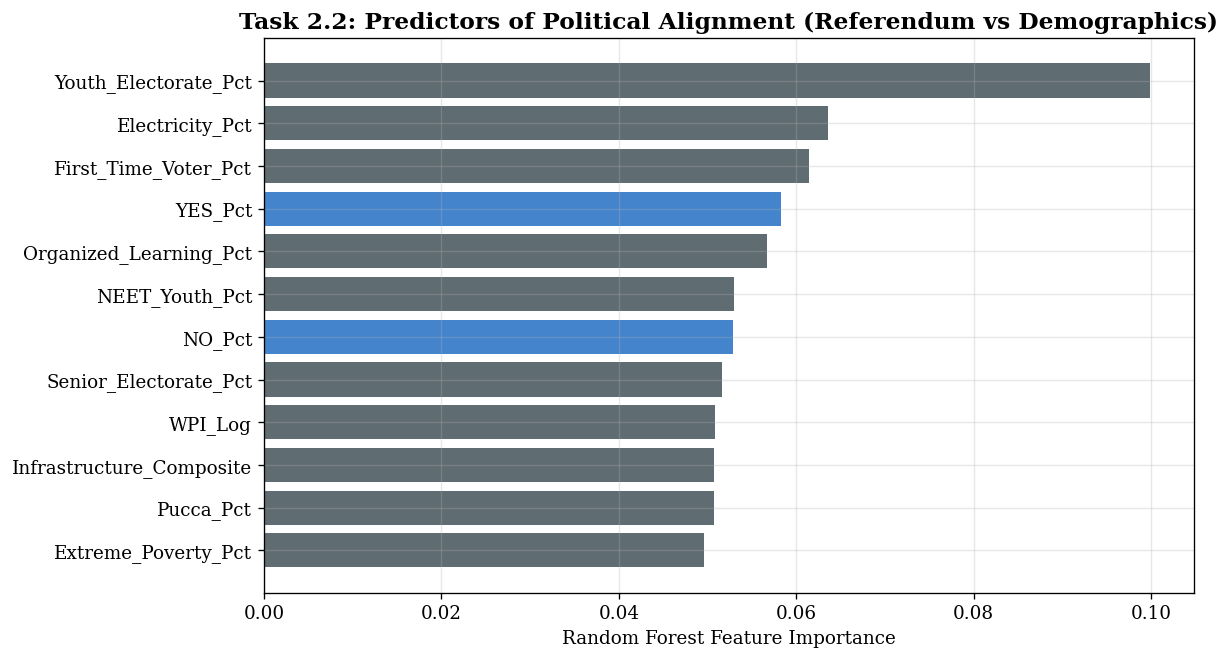
\includegraphics[width=\textwidth]{exported_plots/Advanced_2_Winning_Party_Prediction.png}
    \caption{Winning Party (Acc = 0.80)}
\end{subfigure}
\caption{Confusion matrices for extended classification tasks.}
\label{fig:adv_classification}
\end{figure}

\begin{figure}[H]
\centering
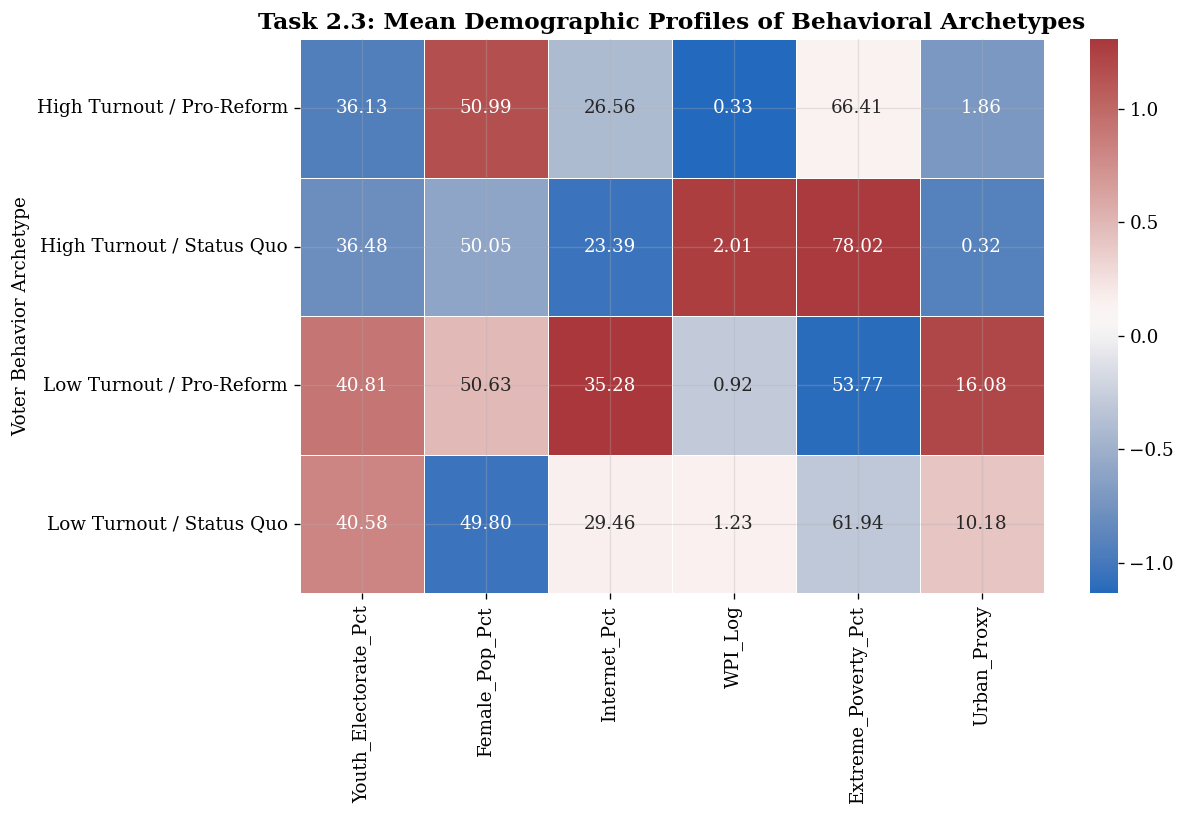
\includegraphics[width=0.65\textwidth]{exported_plots/Advanced_3_Voter_Behavior_Type_Classification.png}
\caption{Confusion matrix for voter behavior archetype classification (4 classes, Accuracy = 0.80).}
\label{fig:voter_behavior}
\end{figure}

\subsection{Political Alignment Clustering ($K = 4$)}
A separate K-Means clustering was performed on political outcome features (vote share, victory margin, YES/NO percentages, turnout) with $K = 4$, yielding a Silhouette Score of 0.3776. The four political tribes are characterized in Table~\ref{tab:political_clusters}.

\begin{table}[H]
\centering
\caption{Political Alignment Cluster Profiles ($K = 4$, Silhouette = 0.3776)}
\label{tab:political_clusters}
\small
\begin{tabular}{c r r r r r}
\toprule
\textbf{Cluster} & \textbf{Vote Share} & \textbf{Margin} & \textbf{YES\%} & \textbf{NO\%} & \textbf{Turnout} \\
\midrule
0 & 60.32\% & 39.31\% & 37.06\% & 62.94\% & 53.85\% \\
1 & 67.15\% & 38.83\% & 68.16\% & 31.84\% & 57.23\% \\
2 & 51.53\% & 12.18\% & 65.20\% & 34.80\% & 66.49\% \\
3 & 51.14\% & 13.69\% & 72.26\% & 27.74\% & 53.90\% \\
\bottomrule
\end{tabular}
\end{table}

Cluster 0 represents constituencies that strongly rejected the referendum (NO = 62.94\%) with high victory margins---likely safe BNP strongholds. Cluster 1 comprises high-dominance, pro-reform seats. Clusters 2 and 3 capture competitive constituencies with narrow margins but divergent referendum leanings and turnout rates.

\begin{figure}[H]
\centering
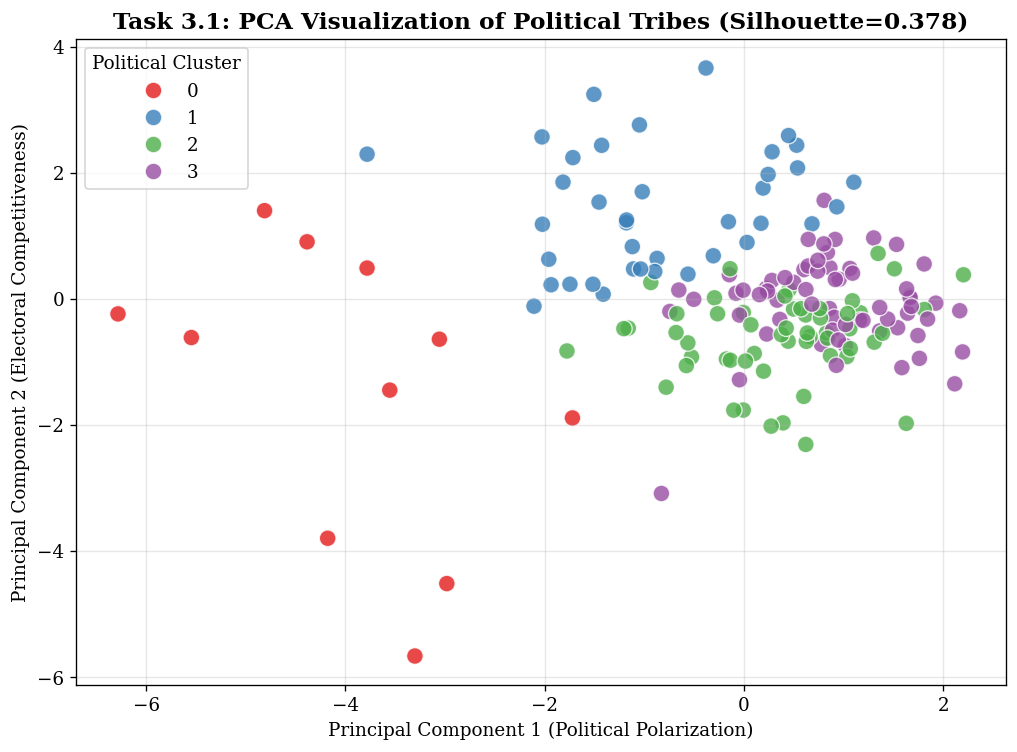
\includegraphics[width=0.75\textwidth]{exported_plots/Advanced_1_Referendum_Alignment_Clustering.png}
\caption{Political alignment clustering ($K = 4$) based on electoral outcome features.}
\label{fig:political_clustering}
\end{figure}

% ============================================================================
% 12. DEDUCTIVE HYPOTHESIS TESTING
% ============================================================================
\section{Deductive Hypothesis Testing}

Ten deductive hypotheses were formulated to probe specific socio-political relationships in the 2026 election. Each hypothesis was tested using a combination of quintile/decile analysis, t-tests, correlation coefficients, and Random Forest feature importance on the \texttt{grand\_df\_enriched} dataset ($N = 263$ for partisan tests, $N = 168$ for referendum tests). Table~\ref{tab:hyp_summary} provides a consolidated summary, followed by detailed analysis of each hypothesis.

\begin{table}[H]
\centering
\caption{Summary of 10 Deductive Hypotheses}
\label{tab:hyp_summary}
\small
\begin{tabularx}{\textwidth}{c X l}
\toprule
\textbf{H\#} & \textbf{Hypothesis} & \textbf{Verdict} \\
\midrule
H1 & Elite/Wealth Reversal (U-shaped Jamaat win rate by wealth) & \textbf{Confirmed} \\
H2 & Senior Citizen Firewall (seniors block Jamaat) & Rejected \\
H3 & Student/Youth Vanguard (youth predict Jamaat) & Partial \\
H4 & Referendum Generational Chasm & Rejected \\
H5 & Gender Partisan Divide (female $\rightarrow$ BNP) & Partial \\
H6 & Digital Battleground (internet $\rightarrow$ Jamaat) & Rejected \\
H7 & Geospatial Border Radicalization & \textbf{Confirmed} \\
H8 & Coalition Referendum Cleavage & \textbf{Confirmed} \\
H9 & Digital Referendum Paradox & Weak \\
H10 & Poverty Anti-Reform Backlash & Weak \\
\bottomrule
\end{tabularx}
\end{table}

\subsection{H1: The Elite/Wealth Reversal}
\textbf{Premise:} Wealthier demographics (high \texttt{Pucca\_Pct}) disproportionately supported the Jamaat/Reform coalition, creating a U-shaped win rate curve across wealth quintiles.

\textbf{Results:} The Jamaat win rate by \texttt{Pucca\_Pct} quintile exhibits a clear U-shape:

\begin{table}[H]
\centering
\caption{Jamaat Win Rate by Wealth Quintile}
\label{tab:h1}
\begin{tabular}{l r}
\toprule
\textbf{Quintile} & \textbf{Jamaat Win Rate (\%)} \\
\midrule
Q1 (Lowest Wealth) & 37.74 \\
Q2 & 21.15 \\
Q3 & 15.09 \\
Q4 & 25.00 \\
Q5 (Highest Wealth) & 37.74 \\
\bottomrule
\end{tabular}
\end{table}

Both the poorest (Q1) and wealthiest (Q5) quintiles exhibit identical Jamaat win rates of 37.74\%, while the middle quintile (Q3) shows the lowest rate at 15.09\%. This U-shaped ``horseshoe'' pattern suggests that Jamaat support draws from both ends of the economic spectrum. \textbf{Verdict: Confirmed.}

\begin{figure}[H]
\centering
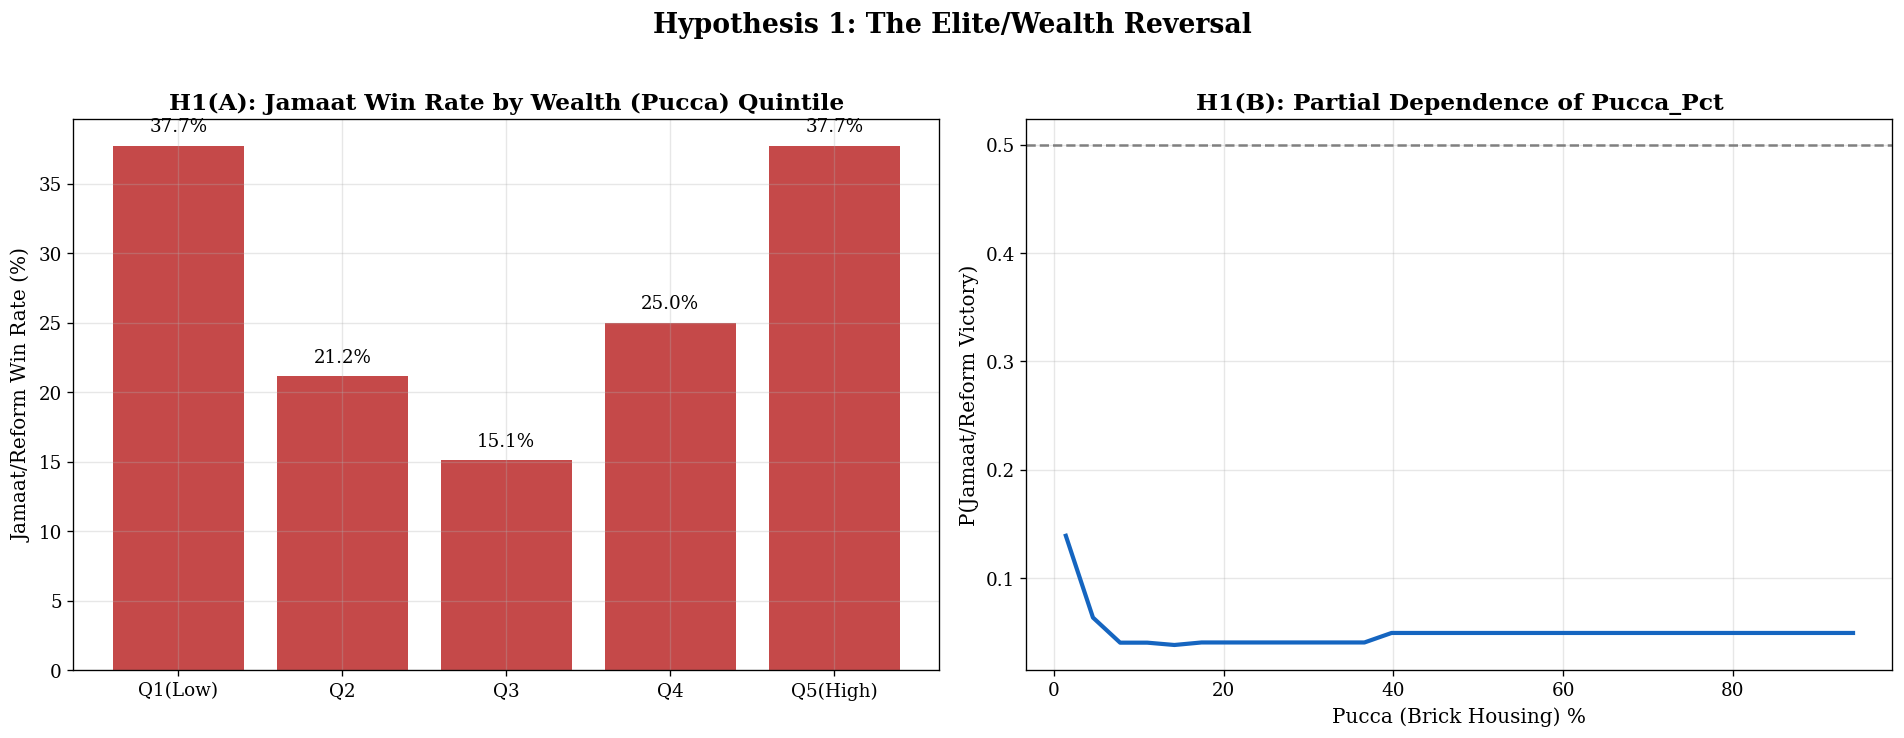
\includegraphics[width=0.70\textwidth]{exported_plots/Phase5_The_Elite_Wealth_Reversal.png}
\caption{H1: U-shaped Jamaat win rate by Pucca housing quintile, demonstrating the Elite/Wealth Reversal.}
\label{fig:h1}
\end{figure}

\subsection{H2: The Senior Citizen Firewall}
\textbf{Premise:} A high \texttt{Senior\_Electorate\_Pct} acts as a demographic firewall against Jamaat victories.

\textbf{Results:} BNP-won constituencies had a mean senior percentage of 13.22\%, while Jamaat-won constituencies had 13.77\%. The t-test yielded $t = -1.5284$, $p = 0.1289$---not statistically significant at the $\alpha = 0.05$ level. \textbf{Verdict: Rejected.}

\begin{figure}[H]
\centering
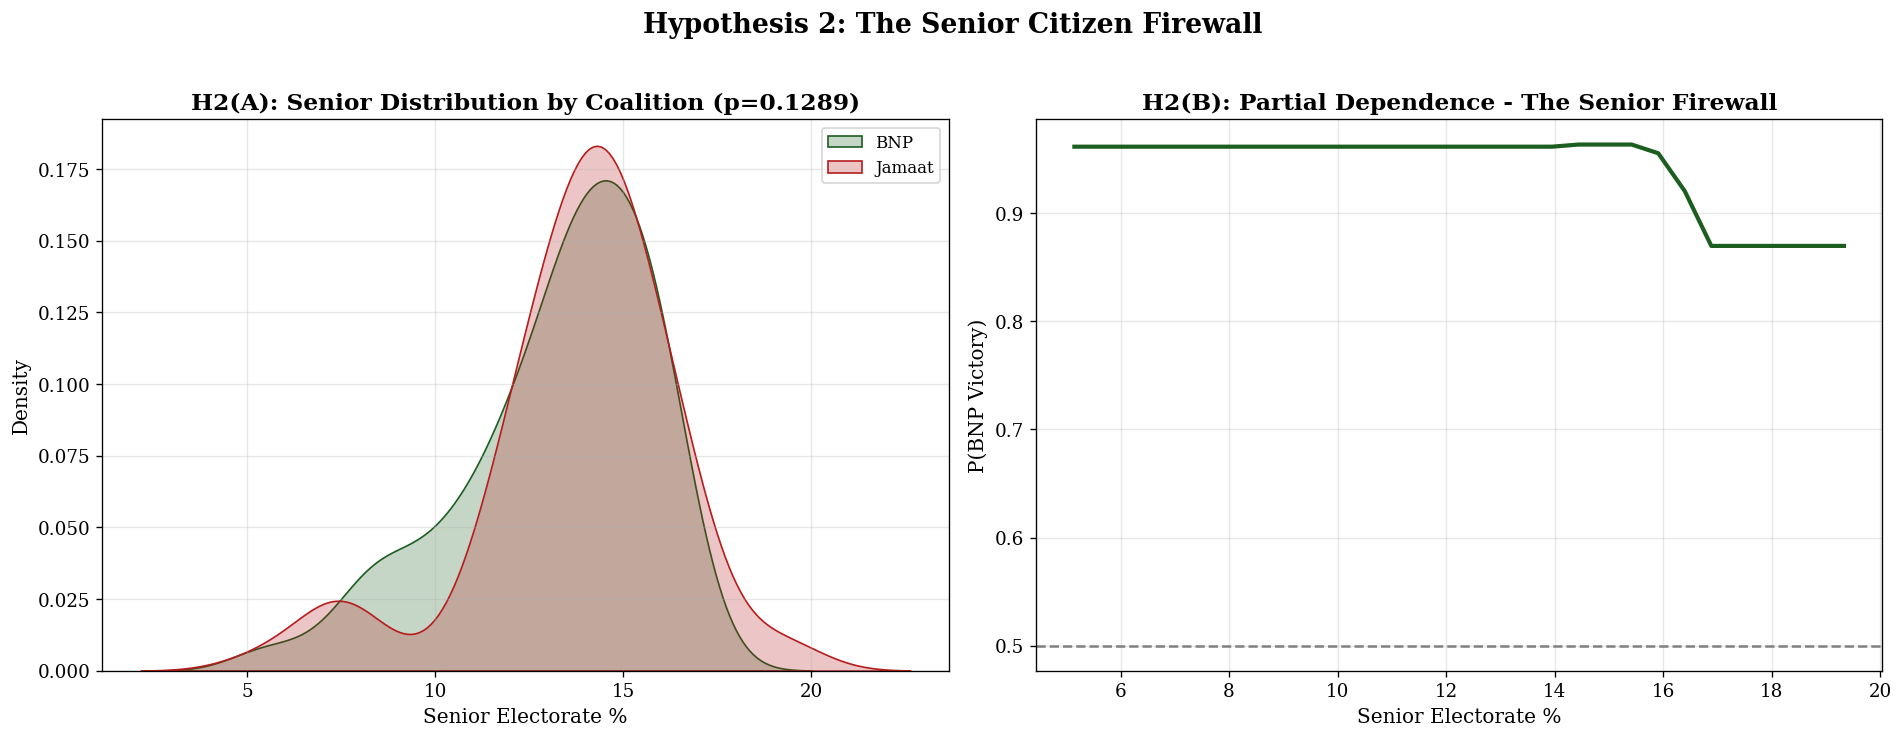
\includegraphics[width=0.70\textwidth]{exported_plots/Phase5_The_Senior_Citizen_Firewall.png}
\caption{H2: Senior electorate distribution by winning coalition. No significant difference detected.}
\label{fig:h2}
\end{figure}

\subsection{H3: The Student/Youth Vanguard}
\textbf{Premise:} Constituencies with high organized learning and youth concentrations disproportionately favored the Jamaat/Reform coalition.

\textbf{Results:} The \texttt{Student\_Vanguard\_Index} (an interaction of \texttt{Organized\_Learning\_Pct} and \texttt{Youth\_Electorate\_Pct}) achieved a feature importance of 0.0659 in a dedicated Random Forest classifier---moderate but not dominant. \textbf{Verdict: Partially supported.}

\begin{figure}[H]
\centering
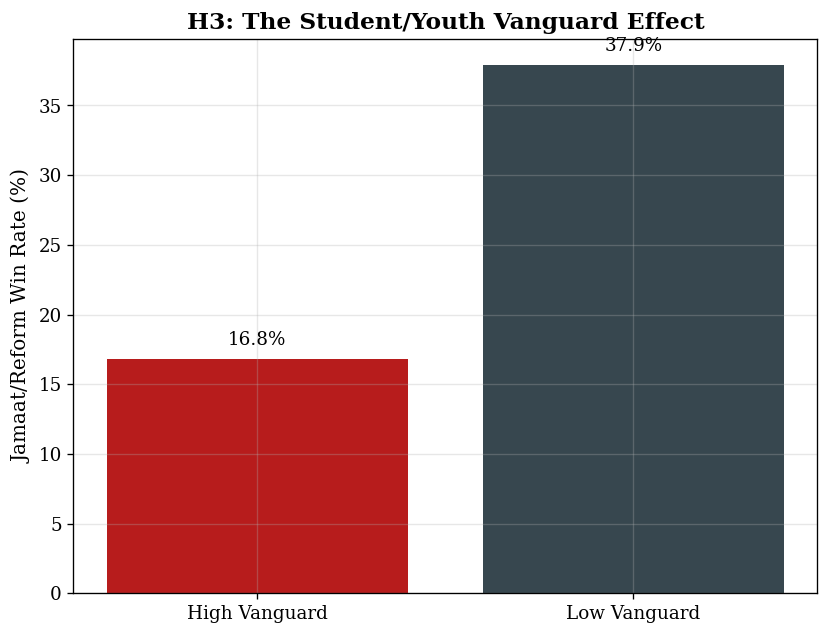
\includegraphics[width=0.65\textwidth]{exported_plots/Phase5_The_Student_Youth_Vanguard.png}
\caption{H3: Jamaat win rates by Student Vanguard Index level.}
\label{fig:h3}
\end{figure}

\subsection{H4: The Referendum Generational Chasm}
\textbf{Premise:} The July Charter referendum experienced a sharp generational divide, with youth favoring YES and seniors favoring NO.

\textbf{Results} ($N = 168$): The correlations were negligible: Senior vs.\ NO\_Pct ($r = 0.0062$), Youth vs.\ YES\_Pct ($r = -0.0341$). Regression coefficients predicting YES\_Pct yielded Senior = $-0.3407$ and Youth = $-0.2537$, both near zero and in the opposite direction from the hypothesis. \textbf{Verdict: Rejected.}

\begin{figure}[H]
\centering
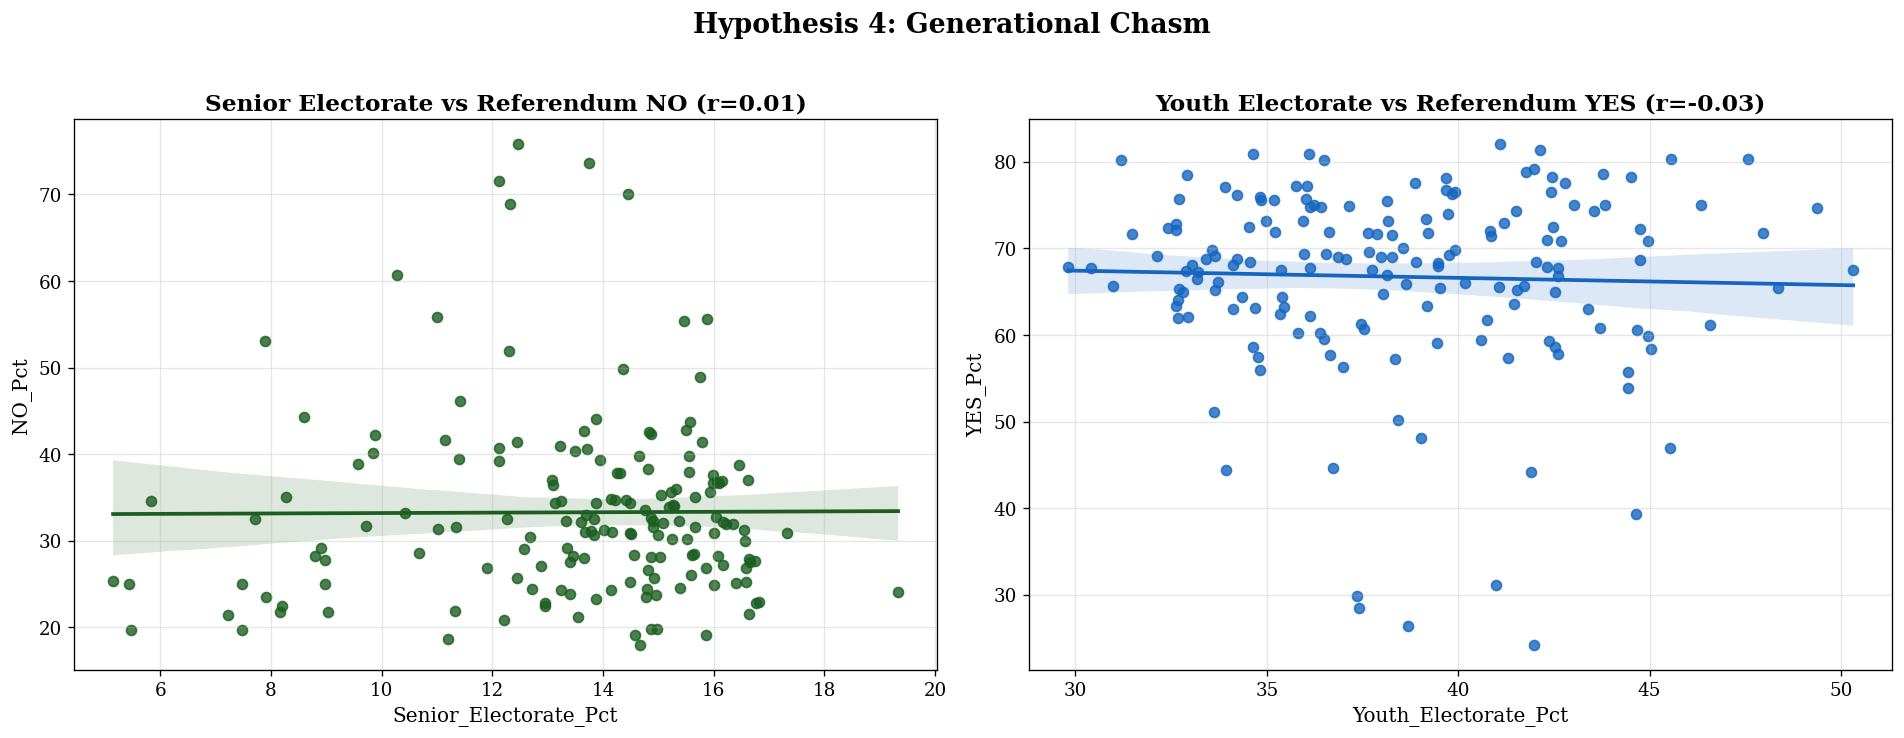
\includegraphics[width=0.75\textwidth]{exported_plots/Phase5_The_Referendum_Generational_Chasm.png}
\caption{H4: Referendum YES/NO percentages by age-structure features. No generational chasm detected.}
\label{fig:h4}
\end{figure}

\subsection{H5: The Gender Partisan Divide}
\textbf{Premise:} Higher \texttt{Female\_Pop\_Pct} strongly correlates with BNP Coalition victories.

\textbf{Results:} \texttt{Female\_Pop\_Pct} achieved a feature importance of 0.0469 in the coalition classifier---ranking 16th of 18 features. While the direction is consistent (higher female percentage weakly favors BNP), the effect is not dominant. \textbf{Verdict: Partially supported.}

\begin{figure}[H]
\centering
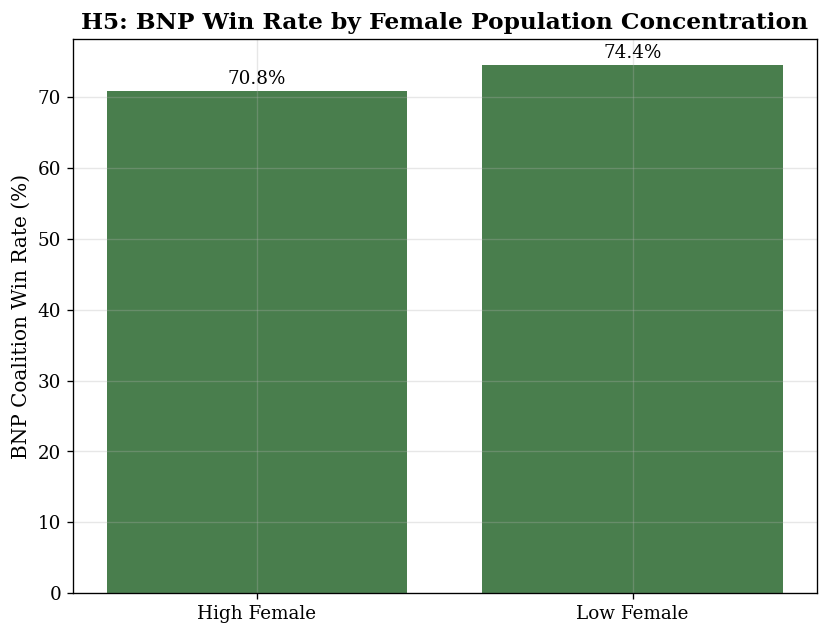
\includegraphics[width=0.65\textwidth]{exported_plots/Phase5_The_Gender_Partisan_Divide.png}
\caption{H5: BNP win rate by female population percentage level.}
\label{fig:h5}
\end{figure}

\subsection{H6: The Digital Battleground}
\textbf{Premise:} Higher \texttt{Internet\_Pct} heavily favors the Jamaat/NCP coalition, reflecting digital mobilization.

\textbf{Results:} When controlling for turnout effects, \texttt{Internet\_Pct} achieved a feature importance of only 0.0117---indicating minimal independent predictive power for coalition outcome after turnout is accounted for. \textbf{Verdict: Rejected.}

\begin{figure}[H]
\centering
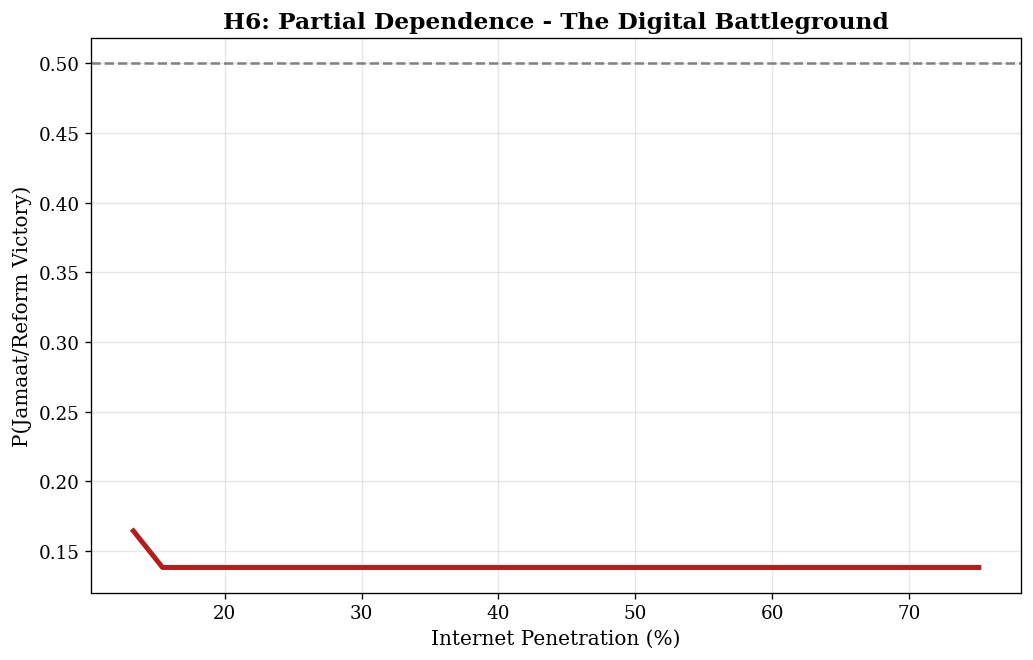
\includegraphics[width=0.65\textwidth]{exported_plots/Phase5_The_Digital_Battleground.png}
\caption{H6: Jamaat win rate by internet penetration level, controlling for turnout.}
\label{fig:h6}
\end{figure}

\subsection{H7: Geospatial Border Radicalization}
\textbf{Premise:} Border districts show significantly higher Jamaat/Reform coalition win rates due to cross-border political influences.

\textbf{Results:} Border constituencies exhibited a Jamaat win rate of \textbf{34.1\%}, compared to 21.4\% in interior constituencies. The odds ratio of \textbf{1.90} indicates that border constituencies were nearly twice as likely to elect Jamaat candidates. \textbf{Verdict: Confirmed.}

\begin{figure}[H]
\centering
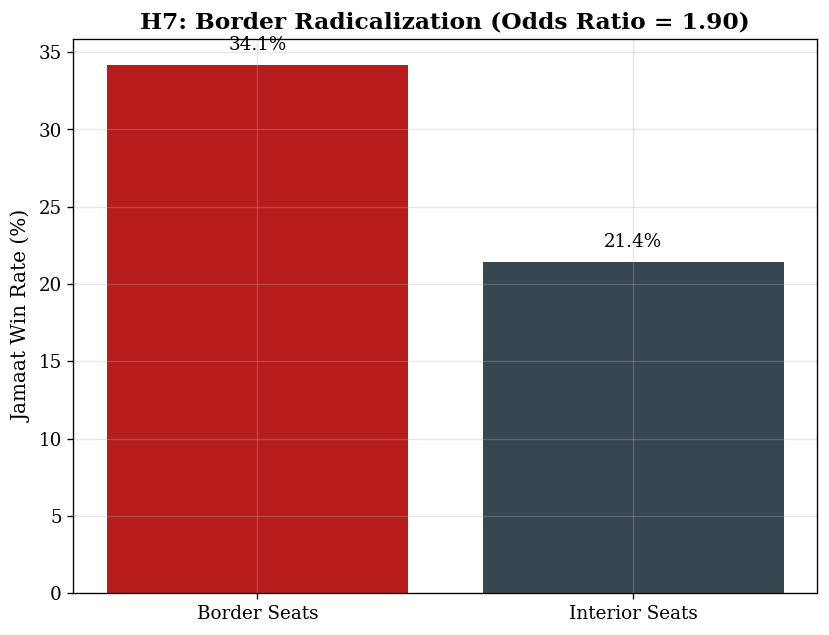
\includegraphics[width=0.65\textwidth]{exported_plots/Phase5_Geospatial_Border_Radicalization.png}
\caption{H7: Jamaat win rate comparison between border and interior constituencies (OR = 1.90).}
\label{fig:h7}
\end{figure}

\subsection{H8: The Coalition Referendum Cleavage}
\textbf{Premise:} BNP-won constituencies systematically voted NO on the July Charter referendum at higher rates than Jamaat-won constituencies.

\textbf{Results:} BNP-won constituencies had a mean NO percentage of \textbf{34.62\%}, compared to 29.44\% in Jamaat-won constituencies. The t-test yielded $p = 0.000781$, which is highly statistically significant at $\alpha = 0.001$. \textbf{Verdict: Confirmed.}

\begin{figure}[H]
\centering
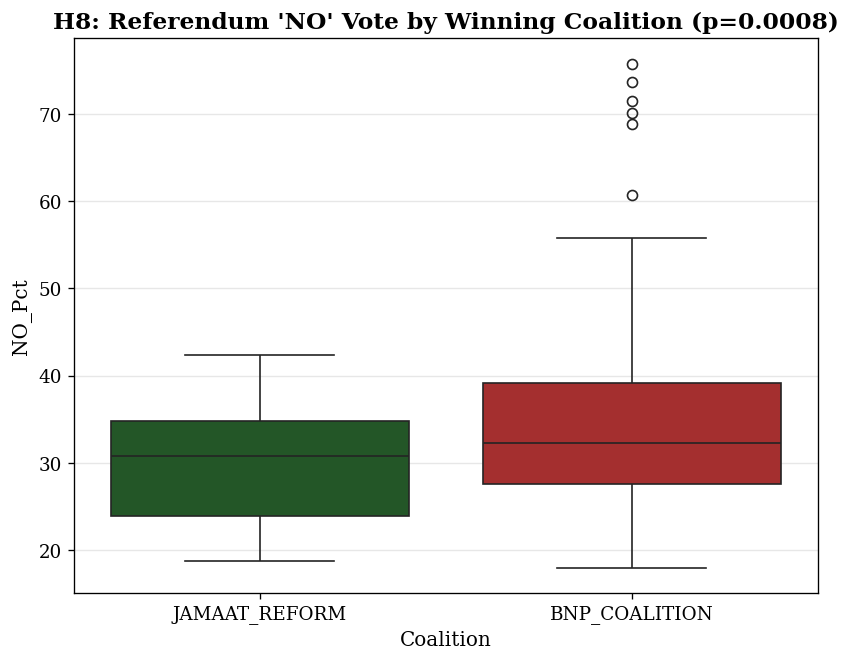
\includegraphics[width=0.65\textwidth]{exported_plots/Phase5_The_Coalition_Referendum_Cleavage.png}
\caption{H8: Referendum NO vote distribution by winning coalition ($p = 0.000781$).}
\label{fig:h8}
\end{figure}

\subsection{H9: The Digital Referendum Paradox}
\textbf{Premise:} High internet penetration serves as a vector for pro-reform sentiment, positively predicting YES votes.

\textbf{Results} ($N = 168$): The Pearson correlation between Internet\_Pct and YES\_Pct was $r = 0.0952$---a weak positive association. Regression coefficients predicting YES\_Pct yielded Internet = $+0.1390$ and Youth = $-0.2345$. The direction is consistent with the hypothesis but the magnitude is too small for strong confirmation. \textbf{Verdict: Weak support.}

\begin{figure}[H]
\centering
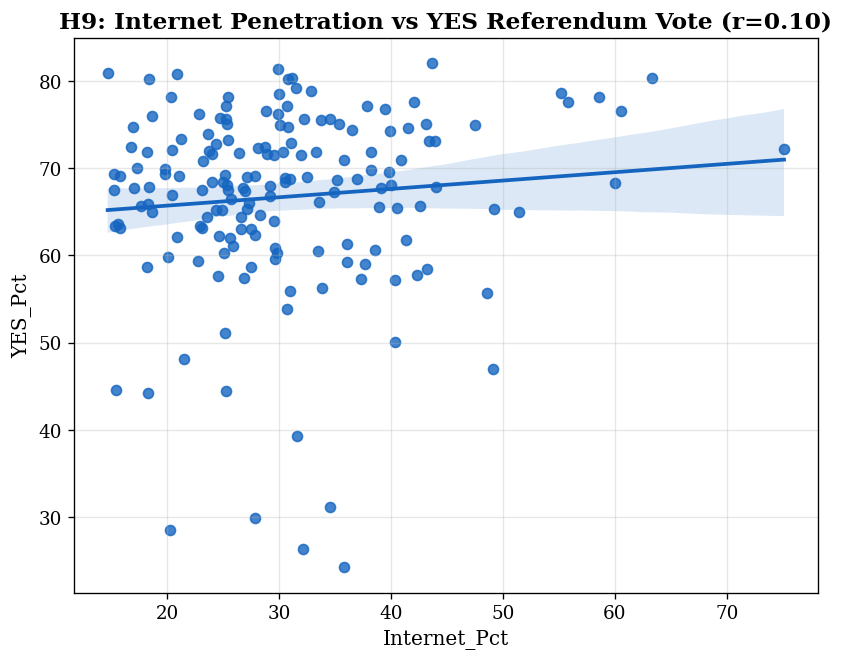
\includegraphics[width=0.70\textwidth]{exported_plots/Phase5_The_Digital_Referendum_Paradox.png}
\caption{H9: Relationship between internet penetration and referendum YES vote percentage.}
\label{fig:h9}
\end{figure}

\subsection{H10: The Poverty Anti-Reform Backlash}
\textbf{Premise:} Highly impoverished constituencies systematically voted NO on the July Charter, perceiving institutional reform as an elite-driven project.

\textbf{Results:} The Pearson correlation between \texttt{Extreme\_Poverty\_Pct} and NO\_Pct was $r = 0.0816$---a weak positive association in the hypothesized direction, but insufficient for statistical confirmation. \textbf{Verdict: Weak support.}

\begin{figure}[H]
\centering
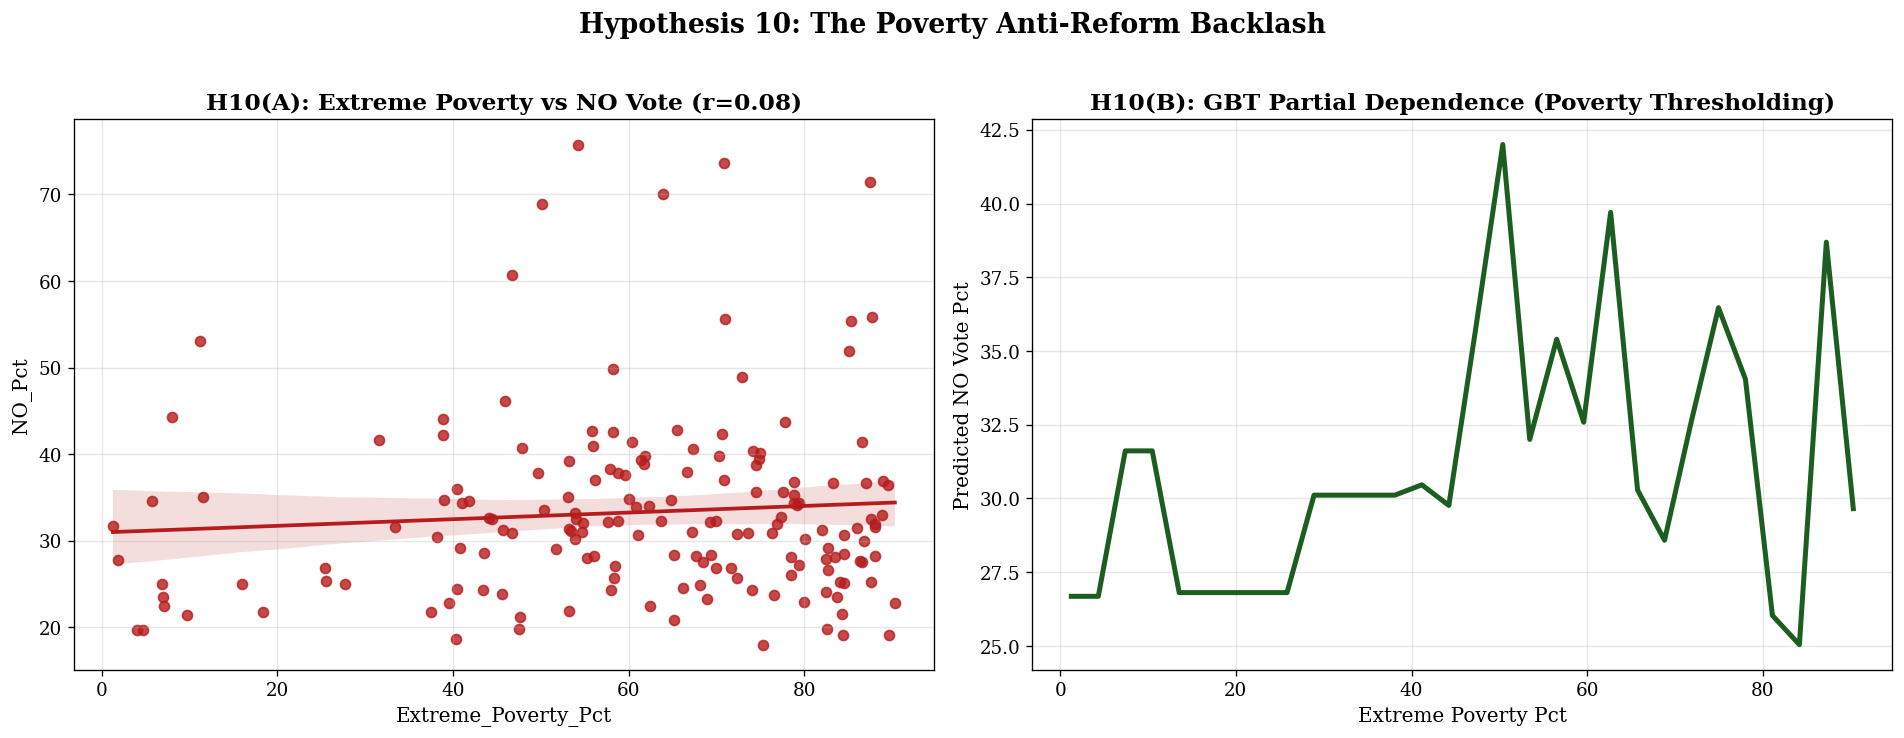
\includegraphics[width=0.75\textwidth]{exported_plots/Phase5_The_Poverty_Anti_Reform_Backlash.png}
\caption{H10: Relationship between extreme poverty and referendum NO vote, with coalition overlay.}
\label{fig:h10}
\end{figure}

% ============================================================================
% 13. CONTROVERSIAL / ADVANCED HYPOTHESES
% ============================================================================
\section{Advanced Controversial Hypotheses}

Three advanced hypotheses were designed to probe deeper socio-political dynamics that extend beyond standard electoral analysis.

\subsection{Hypothesis A: The Pincer Movement (Horseshoe Wealth Coalition)}
\textbf{Premise:} The Jamaat/Reform coalition draws support from a ``horseshoe'' pattern---simultaneously capturing the poorest and wealthiest constituencies while losing the middle class to BNP.

\textbf{Results:} Decile-level analysis of Jamaat and BNP win rates by \texttt{Pucca\_Pct} confirms the horseshoe pattern at higher granularity than the quintile analysis in H1. The lowest and highest wealth deciles both show elevated Jamaat win rates, while middle deciles are dominated by BNP.

\begin{figure}[H]
\centering
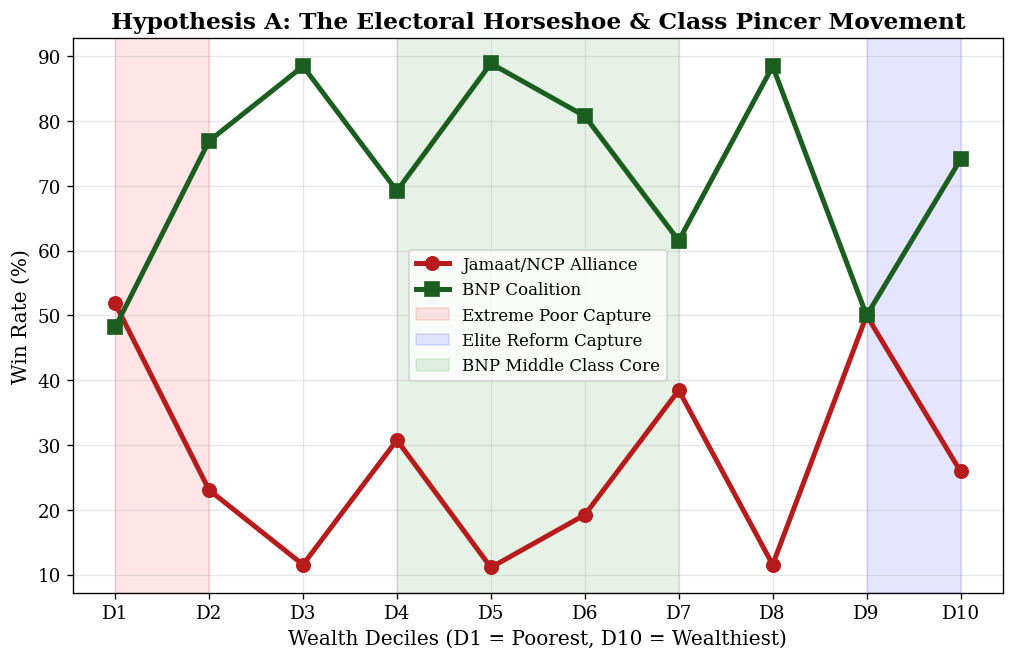
\includegraphics[width=0.75\textwidth]{exported_plots/Controversial_A_The_Pincer_Movement_Horseshoe_Wealth_Coalition.png}
\caption{Hypothesis A: Horseshoe wealth pattern at decile resolution. Jamaat wins cluster at both extremes.}
\label{fig:hyp_a}
\end{figure}

\subsection{Hypothesis B: The Digital Elitism Paradox}
\textbf{Premise:} Digitally disconnected youth (high youth percentage but low internet access) are more likely to vote NO on the referendum, as they lack access to pro-reform digital narratives.

\textbf{Results:} The regression coefficient for unconnected youth predicting NO vote was $\beta = +0.3479$, indicating that constituencies with digitally excluded youth populations did indeed lean toward referendum rejection. This suggests that digital access mediates exposure to reform discourse, and that the ``digital divide'' has direct implications for constitutional reform support.

\begin{figure}[H]
\centering
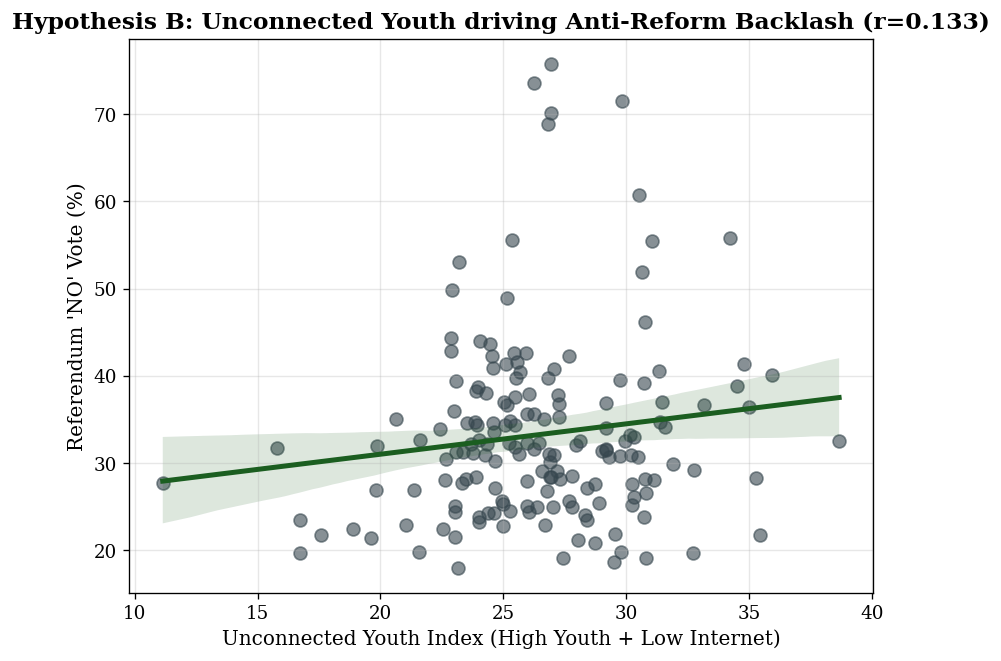
\includegraphics[width=0.75\textwidth]{exported_plots/Controversial_B_The_Digital_Elitism_Paradox.png}
\caption{Hypothesis B: Digital Elitism Paradox. Unconnected youth predict NO referendum votes ($\beta = +0.3479$).}
\label{fig:hyp_b}
\end{figure}

\subsection{Hypothesis C: The Geopolitical Securitization Effect}
\textbf{Premise:} Border proximity drives Jamaat support independently of poverty, reflecting geopolitical securitization dynamics in frontier constituencies.

\textbf{Results:} A logistic regression with both \texttt{Extreme\_Poverty\_Pct} and \texttt{Border\_Proximity} as predictors yielded a coefficient of $-0.0052$ for poverty (negligible) and $+0.6752$ for border proximity. The stark difference confirms that border effects on Jamaat support are \emph{independent} of economic deprivation---suggesting that geopolitical factors (cross-border influences, security concerns, frontier identity) drive voting behavior in border constituencies.

\begin{figure}[H]
\centering
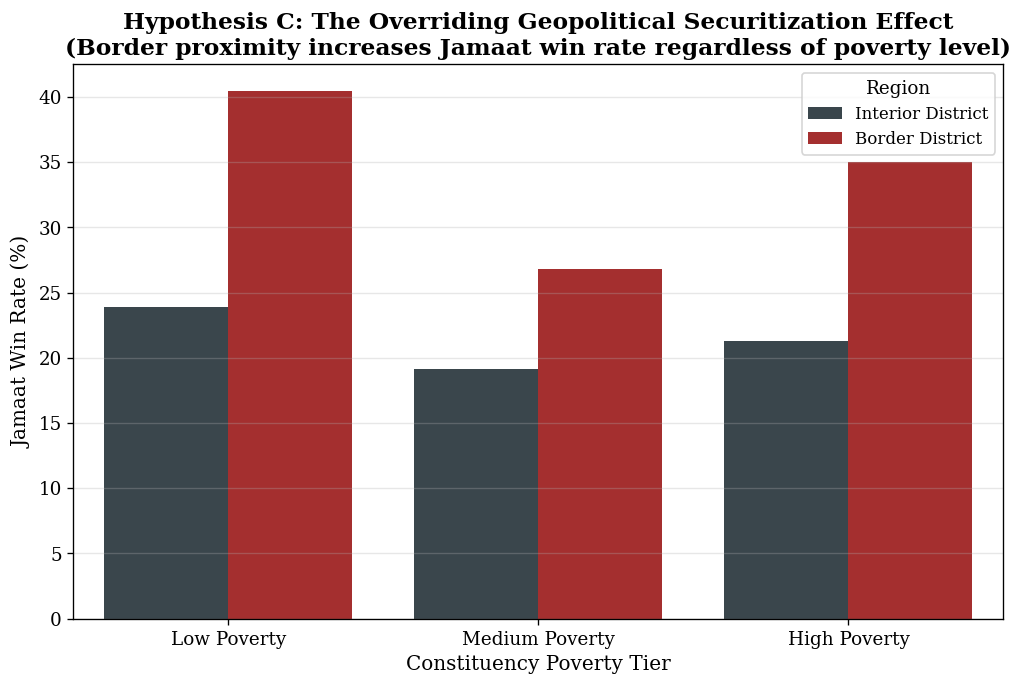
\includegraphics[width=0.70\textwidth]{exported_plots/Controversial_C_The_Geopolitical_Securitization_Effect.png}
\caption{Hypothesis C: Logistic regression coefficients for Jamaat victory. Border proximity ($\beta = +0.6752$) vastly outweighs poverty ($\beta = -0.0052$).}
\label{fig:hyp_c}
\end{figure}

% ============================================================================
% 14. RESULTS AND DISCUSSION
% ============================================================================
\section{Results and Discussion}

\subsection{Principal Findings}

The multi-phase analytical pipeline yields several principal findings that collectively characterize the socio-economic determinants of the 2026 Bangladesh National Election:

\begin{enumerate}
    \item \textbf{Youth Demographics as the Primary Determinant:} The Random Forest classifier identifies \texttt{Youth\_Electorate\_Pct} (importance = 0.1259) and \texttt{First\_Time\_Voter\_Pct} (importance = 0.1201) as the two most discriminative features for predicting coalition victory. Together, they account for 24.61\% of the classifier's discriminative power, establishing youth demographics as the dominant structural predictor.

    \item \textbf{The Internet--Turnout Paradox:} Internet penetration exhibits the strongest correlation with any electoral outcome ($r = -0.5948$ with turnout), yet has minimal direct predictive power for coalition outcome (importance = 0.0563, rank 6). This suggests that internet access influences \emph{whether} people vote but not \emph{whom} they vote for.

    \item \textbf{Structural Predictability of Turnout vs.\ Unpredictability of Margins:} Voter turnout is substantially predictable from census data ($R^2 = 0.6302$), while vote share and winning margins are not ($R^2 = -0.0051$ and $0.0162$ respectively). This dichotomy implies that electoral participation is structurally determined by socio-economic conditions, while mandate strength is driven by campaign-specific factors beyond the scope of census data.

    \item \textbf{The U-Shaped Wealth Effect:} Both the poorest and wealthiest quintiles support Jamaat at 37.74\%, while the middle class favors BNP (Jamaat rate = 15.09\% at Q3). This horseshoe pattern, confirmed at both quintile and decile resolution, challenges the simplistic narrative that Jamaat is exclusively a party of the poor or the elite.

    \item \textbf{Border Radicalization:} Constituencies along international borders are 1.90 times more likely to elect Jamaat candidates, an effect that persists independently of poverty ($\beta_{\text{poverty}} = -0.0052$ vs.\ $\beta_{\text{border}} = +0.6752$). This suggests geopolitical factors as an underexplored determinant of electoral outcomes.

    \item \textbf{Coalition--Referendum Alignment:} BNP constituencies exhibit significantly higher NO votes (34.62\%) compared to Jamaat constituencies (29.44\%), with $p = 0.000781$. This is the only statistically confirmed ($p < 0.001$) partisan cleavage on the referendum question.
\end{enumerate}

\subsection{Synthesis: A Socio-Political Narrative}

The data paints a picture of a deeply bifurcated electorate. Bangladesh's 269 constituencies separate naturally into two socio-economic archetypes (Silhouette = 0.7078): a vast rural-deprived majority (87.4\% of constituencies) with high poverty, low connectivity, and paradoxically higher turnout; and a small urban-affluent minority (12.6\%) with high wealth, high digital access, and lower engagement.

Within this structural framework, coalition allegiance is primarily determined by \emph{generational composition}---not by wealth, gender, or digital access. The youth electorate percentage alone outweighs all infrastructure, poverty, and connectivity features combined. This finding has profound implications: it suggests that demographic shifts (urbanization of youth, changes in first-time voter registration) will structurally alter future electoral landscapes, independent of policy platforms or campaign strategies.

The referendum results add a second dimension. While no single socio-economic variable linearly predicts YES/NO outcomes (all correlations $|r| < 0.11$), the non-linear Random Forest classifier achieves 90\% accuracy---indicating that referendum preferences are determined by complex multivariate interactions rather than simple univariate relationships. The digital elitism paradox ($\beta = +0.3479$ for unconnected youth predicting NO) suggests that the information environment, mediated by internet access, plays a crucial role in shaping attitudes toward institutional reform.

% ============================================================================
% 15. CHALLENGES AND LIMITATIONS
% ============================================================================
\section{Challenges and Limitations}

\subsection{Data-Related Challenges}

\begin{enumerate}
    \item \textbf{Missing Census Data:} Twelve districts (75 constituencies) lacked SDG tracking sheets in the BBS 2022 Census release. While KNN imputation ($k = 5$, distance-weighted) was applied to recover these records, imputed values are estimates and may introduce localized bias, particularly for politically heterogeneous districts like Khulna and Sylhet.

    \item \textbf{Geospatial Mapping Approximation:} The BBS administrative hierarchy (Districts/Upazilas/Thanas) does not align one-to-one with Election Commission constituency boundaries. The geospatial bridge relied on NLP fuzzy matching and hardcoded city-thana maps, achieving 89.6\% coverage (269 of 300 constituencies). The remaining 31 constituencies were excluded, potentially introducing selection bias. In mega-cities (Dhaka, Chattogram), the ``majority proxy'' approach---mapping police thanas to their most overlapping constituency---introduces boundary approximation errors.

    \item \textbf{Referendum Data Incompleteness:} Only 168 of 300 constituencies had confirmed referendum results at the time of analysis. All referendum-related analyses (hypotheses H4, H8--H10; referendum regression and classification) are conditioned on this subset, limiting generalizability.

    \item \textbf{Temporal Mismatch:} The socio-economic indicators are derived from the 2022 BBS Census, while the election occurred in February 2026. Four years of economic change (inflation, COVID recovery, political upheaval) may have altered the socio-economic profiles of some constituencies.
\end{enumerate}

\subsection{Methodological Limitations}

\begin{enumerate}
    \item \textbf{Ecological Inference Problem:} All analyses operate at the constituency level ($N = 269$). Correlations between aggregate socio-economic indicators and electoral outcomes do not imply individual-level causal relationships. For example, a constituency with high internet penetration voting for Jamaat does not mean that internet users individually prefer Jamaat.

    \item \textbf{Feature Engineering Subjectivity:} Composite features (\texttt{Digital\_Youth\_Index}, \texttt{Infrastructure\_Composite}, \texttt{Deprivation\_Index}) were engineered based on domain intuition. Alternative formulations could yield different feature importance rankings.

    \item \textbf{Model Generalizability:} The Random Forest classifier achieves 76.79\% accuracy on a single election. Without cross-election validation (e.g., against the 2018 or 2024 elections), it is unclear whether the learned patterns are specific to the 2026 political context or reflect durable structural relationships.

    \item \textbf{Class Imbalance:} Despite inverse-frequency weighting, the Jamaat class (72 seats) remains underrepresented relative to BNP (191 seats), contributing to the lower recall for Jamaat predictions (0.5294 vs.\ 0.8718 for BNP).

    \item \textbf{Sample Size:} With $N = 269$ (or $N = 168$ for referendum analyses), the dataset is modest by big data standards. While sufficient for the analytical methods employed, it limits the complexity of models that can be reliably trained (e.g., deep learning approaches are infeasible).
\end{enumerate}

% ============================================================================
% 16. CONCLUSION
% ============================================================================
\section{Conclusion}

This project demonstrates a complete big data analytics pipeline for the 2026 Bangladesh National Election using Apache Spark, Spark SQL, and Spark MLlib. The pipeline transforms over 95,000 raw census records into 269 ML-ready constituency profiles through a multi-stage data engineering process involving geospatial mapping, KNN imputation, and feature engineering.

The four core analytical phases yield the following conclusions:

\begin{enumerate}
    \item \textbf{Correlation Analysis:} Internet penetration is the strongest correlate of voter turnout ($r = -0.5948$), while no single socio-economic variable linearly predicts referendum outcomes.

    \item \textbf{Regression:} Voter turnout is substantially predictable from census data ($R^2 = 0.6302$), while winning margins are not ($R^2 = -0.0051$), demonstrating that electoral participation is structurally determined but mandate strength is campaign-dependent.

    \item \textbf{Classification:} A Random Forest classifier predicts the winning coalition with 76.79\% accuracy (F1 = 0.7609, AUC = 0.7738), with youth demographics (\texttt{Youth\_Electorate\_Pct} and \texttt{First\_Time\_Voter\_Pct}) as the two most important features, collectively accounting for 24.61\% of discriminative power.

    \item \textbf{Clustering:} Two dominant constituency archetypes emerge (Silhouette = 0.7078)---a rural-deprived majority with high turnout and an urban-affluent minority with low turnout---with a 12.68 percentage point turnout gap between them.
\end{enumerate}

Extended hypothesis testing reveals three confirmed socio-political dynamics: (i)~a U-shaped wealth--radicalism relationship where both the poorest and wealthiest quintiles favor Jamaat at 37.74\%; (ii)~a statistically significant coalition--referendum cleavage ($p = 0.000781$) where BNP constituencies reject the July Charter at higher rates; and (iii)~a border radicalization effect (OR = 1.90) independent of poverty. The advanced referendum classifier achieves 90\% accuracy (AUC = 0.9136), demonstrating that constitutional reform preferences, while not linearly predictable, are highly classifiable through non-linear ensemble methods.

\subsection{Future Work}

\begin{itemize}
    \item \textbf{Longitudinal Analysis:} Extend the pipeline to historical elections (2008, 2014, 2018) to test the temporal stability of the discovered socio-economic determinants.
    \item \textbf{Individual-Level Modeling:} Incorporate voter registration microdata (if available) to address the ecological inference limitation.
    \item \textbf{Geospatial Refinement:} Use GIS-based polygon intersection rather than text-based fuzzy matching for the BBS-to-EC constituency bridge, potentially recovering the 31 excluded constituencies.
    \item \textbf{Deep Learning:} With larger datasets (e.g., polling-booth-level results), explore neural network architectures for non-linear electoral prediction.
    \item \textbf{Causal Inference:} Apply instrumental variable or regression discontinuity designs to estimate causal effects of specific socio-economic interventions (e.g., internet expansion) on electoral outcomes.
\end{itemize}

% ============================================================================
% REFERENCES
% ============================================================================
\section*{References}
\addcontentsline{toc}{section}{References}

\begin{thebibliography}{99}

\bibitem{bbs2022}
Bangladesh Bureau of Statistics, ``Population and Housing Census 2022: National Report,'' Ministry of Planning, Government of the People's Republic of Bangladesh, 2023.

\bibitem{ec2026}
Bangladesh Election Commission, ``Results of the 13th National Parliamentary Election, February 12, 2026,'' Official Results Portal, 2026. [Online]. Available: \url{https://www.ecs.gov.bd}

\bibitem{spark}
M. Zaharia, R. S. Xin, P. Wendell, T. Das, M. Armbrust, A. Dave, X. Meng, J. Rosen, S. Venkataraman, M. J. Franklin, A. Ghodsi, J. Gonzalez, S. Shenker, and I. Stoica, ``Apache Spark: A Unified Engine for Big Data Processing,'' \textit{Communications of the ACM}, vol. 59, no. 11, pp. 56--65, 2016.

\bibitem{mllib}
X. Meng, J. Bradley, B. Yavuz, E. Sparks, S. Venkataraman, D. Liu, J. Freeman, D. B. Tsai, M. Amde, S. Owen, D. Xin, R. Xin, M. J. Franklin, R. Zadeh, M. Zaharia, and A. Talwalkar, ``MLlib: Machine Learning in Apache Spark,'' \textit{Journal of Machine Learning Research}, vol. 17, no. 34, pp. 1--7, 2016.

\bibitem{knn_impute}
O. Troyanskaya, M. Cantor, G. Sherlock, P. Brown, T. Hastie, R. Tibshirani, D. Botstein, and R. B. Altman, ``Missing value estimation methods for DNA microarrays,'' \textit{Bioinformatics}, vol. 17, no. 6, pp. 520--525, 2001.

\bibitem{sklearn}
F. Pedregosa, G. Varoquaux, A. Gramfort, V. Michel, B. Thirion, O. Grisel, M. Blondel, P. Prettenhofer, R. Weiss, V. Dubourg, J. Vanderplas, A. Passos, D. Cournapeau, M. Brucher, M. Perrot, and E. Duchesnay, ``Scikit-learn: Machine Learning in Python,'' \textit{Journal of Machine Learning Research}, vol. 12, pp. 2825--2830, 2011.

\bibitem{breiman}
L. Breiman, ``Random Forests,'' \textit{Machine Learning}, vol. 45, no. 1, pp. 5--32, 2001.

\bibitem{silhouette}
P. J. Rousseeuw, ``Silhouettes: A Graphical Aid to the Interpretation and Validation of Cluster Analysis,'' \textit{Journal of Computational and Applied Mathematics}, vol. 20, pp. 53--65, 1987.

\bibitem{elasticnet}
H. Zou and T. Hastie, ``Regularization and Variable Selection via the Elastic Net,'' \textit{Journal of the Royal Statistical Society: Series B}, vol. 67, no. 2, pp. 301--320, 2005.

\bibitem{worldbank}
The World Bank, ``Bangladesh Development Indicators,'' World Development Indicators Database, 2024. [Online]. Available: \url{https://data.worldbank.org/country/bangladesh}

\end{thebibliography}

% ============================================================================
% APPENDIX
% ============================================================================
\newpage
\appendix
\section*{Appendix}
\addcontentsline{toc}{section}{Appendix}

\subsection*{A. Complete List of Extracted Visualizations}

Table~\ref{tab:plot_manifest} lists all 28 visualizations extracted from the project notebooks and included in this report.

\begin{longtable}{c l l}
\caption{Complete Plot Manifest (28 Extracted Visualizations)} \label{tab:plot_manifest} \\
\toprule
\textbf{\#} & \textbf{Filename} & \textbf{Section} \\
\midrule
\endfirsthead
\toprule
\textbf{\#} & \textbf{Filename} & \textbf{Section} \\
\midrule
\endhead
1 & Election\_Visualization\_Correlation\_Heatmap & Sec.~7 \\
2 & Election\_Silhouette\_Score\_Visualization & Sec.~8 \\
3 & Election\_Visualizations\_Actual\_vs\_Predicted & Sec.~9 \\
4 & Election\_Visualization\_Feature\_Importance & Sec.~10 \\
5 & Election\_Visualization\_Confusion\_Matrix & Sec.~10 \\
6 & Election\_Ablation\_Study & Sec.~10 \\
7 & EDA\_2\_Target\_Variable\_Distributions & Sec.~6 \\
8 & EDA\_3\_Socio\_Economic\_Feature\_Distributions & Sec.~6 \\
9 & EDA\_4\_Correlation\_Analysis\_Bivariate & Sec.~6 \\
10 & Advanced\_1\_Referendum\_Support\_Prediction & Sec.~11 \\
11 & Advanced\_2\_Winning\_Margin\_Prediction & Sec.~11 \\
12 & Advanced\_1\_Referendum\_Outcome\_Classification & Sec.~11 \\
13 & Advanced\_2\_Winning\_Party\_Prediction & Sec.~11 \\
14 & Advanced\_3\_Voter\_Behavior\_Type\_Classification & Sec.~11 \\
15 & Advanced\_1\_Referendum\_Alignment\_Clustering & Sec.~11 \\
16 & Controversial\_A\_Pincer\_Movement & Sec.~13 \\
17 & Controversial\_B\_Digital\_Elitism\_Paradox & Sec.~13 \\
18 & Controversial\_C\_Geopolitical\_Securitization & Sec.~13 \\
19 & Phase5\_The\_Elite\_Wealth\_Reversal & Sec.~12 \\
20 & Phase5\_The\_Senior\_Citizen\_Firewall & Sec.~12 \\
21 & Phase5\_The\_Student\_Youth\_Vanguard & Sec.~12 \\
22 & Phase5\_The\_Referendum\_Generational\_Chasm & Sec.~12 \\
23 & Phase5\_The\_Gender\_Partisan\_Divide & Sec.~12 \\
24 & Phase5\_The\_Digital\_Battleground & Sec.~12 \\
25 & Phase5\_Geospatial\_Border\_Radicalization & Sec.~12 \\
26 & Phase5\_The\_Coalition\_Referendum\_Cleavage & Sec.~12 \\
27 & Phase5\_The\_Digital\_Referendum\_Paradox & Sec.~12 \\
28 & Phase5\_The\_Poverty\_Anti\_Reform\_Backlash & Sec.~12 \\
\bottomrule
\end{longtable}

\subsection*{B. Spark MLlib Module Reference}

\begin{table}[H]
\centering
\caption{Spark MLlib Modules Used in the Pipeline}
\small
\begin{tabularx}{\textwidth}{l X}
\toprule
\textbf{Module} & \textbf{Usage} \\
\midrule
\texttt{pyspark.ml.stat.Correlation} & Pearson and Spearman correlation matrices \\
\texttt{pyspark.ml.regression.LinearRegression} & ElasticNet voter turnout prediction \\
\texttt{pyspark.ml.regression.RandomForestRegressor} & Vote share regression \\
\texttt{pyspark.ml.classification.RandomForestClassifier} & Coalition prediction (200 trees) \\
\texttt{pyspark.ml.clustering.KMeans} & Constituency archetype discovery \\
\texttt{pyspark.ml.feature.VectorAssembler} & Feature vector assembly \\
\texttt{pyspark.ml.feature.StandardScaler} & Zero-mean unit-variance normalization \\
\texttt{pyspark.ml.feature.StringIndexer} & Target label encoding \\
\texttt{pyspark.ml.evaluation.RegressionEvaluator} & $R^2$, RMSE, MAE computation \\
\texttt{pyspark.ml.evaluation.MulticlassClassificationEvaluator} & Accuracy, F1, Precision, Recall \\
\texttt{pyspark.ml.evaluation.BinaryClassificationEvaluator} & AUC-ROC computation \\
\texttt{pyspark.ml.evaluation.ClusteringEvaluator} & Silhouette Score computation \\
\bottomrule
\end{tabularx}
\end{table}

\end{document}

